% Options for packages loaded elsewhere
\PassOptionsToPackage{unicode}{hyperref}
\PassOptionsToPackage{hyphens}{url}
\PassOptionsToPackage{dvipsnames,svgnames,x11names}{xcolor}
%
\documentclass[
  letterpaper,
  DIV=11,
  numbers=noendperiod]{scrartcl}

\usepackage{amsmath,amssymb}
\usepackage{iftex}
\ifPDFTeX
  \usepackage[T1]{fontenc}
  \usepackage[utf8]{inputenc}
  \usepackage{textcomp} % provide euro and other symbols
\else % if luatex or xetex
  \usepackage{unicode-math}
  \defaultfontfeatures{Scale=MatchLowercase}
  \defaultfontfeatures[\rmfamily]{Ligatures=TeX,Scale=1}
\fi
\usepackage{lmodern}
\ifPDFTeX\else  
    % xetex/luatex font selection
\fi
% Use upquote if available, for straight quotes in verbatim environments
\IfFileExists{upquote.sty}{\usepackage{upquote}}{}
\IfFileExists{microtype.sty}{% use microtype if available
  \usepackage[]{microtype}
  \UseMicrotypeSet[protrusion]{basicmath} % disable protrusion for tt fonts
}{}
\makeatletter
\@ifundefined{KOMAClassName}{% if non-KOMA class
  \IfFileExists{parskip.sty}{%
    \usepackage{parskip}
  }{% else
    \setlength{\parindent}{0pt}
    \setlength{\parskip}{6pt plus 2pt minus 1pt}}
}{% if KOMA class
  \KOMAoptions{parskip=half}}
\makeatother
\usepackage{xcolor}
\setlength{\emergencystretch}{3em} % prevent overfull lines
\setcounter{secnumdepth}{-\maxdimen} % remove section numbering
% Make \paragraph and \subparagraph free-standing
\ifx\paragraph\undefined\else
  \let\oldparagraph\paragraph
  \renewcommand{\paragraph}[1]{\oldparagraph{#1}\mbox{}}
\fi
\ifx\subparagraph\undefined\else
  \let\oldsubparagraph\subparagraph
  \renewcommand{\subparagraph}[1]{\oldsubparagraph{#1}\mbox{}}
\fi

\usepackage{color}
\usepackage{fancyvrb}
\newcommand{\VerbBar}{|}
\newcommand{\VERB}{\Verb[commandchars=\\\{\}]}
\DefineVerbatimEnvironment{Highlighting}{Verbatim}{commandchars=\\\{\}}
% Add ',fontsize=\small' for more characters per line
\usepackage{framed}
\definecolor{shadecolor}{RGB}{241,243,245}
\newenvironment{Shaded}{\begin{snugshade}}{\end{snugshade}}
\newcommand{\AlertTok}[1]{\textcolor[rgb]{0.68,0.00,0.00}{#1}}
\newcommand{\AnnotationTok}[1]{\textcolor[rgb]{0.37,0.37,0.37}{#1}}
\newcommand{\AttributeTok}[1]{\textcolor[rgb]{0.40,0.45,0.13}{#1}}
\newcommand{\BaseNTok}[1]{\textcolor[rgb]{0.68,0.00,0.00}{#1}}
\newcommand{\BuiltInTok}[1]{\textcolor[rgb]{0.00,0.23,0.31}{#1}}
\newcommand{\CharTok}[1]{\textcolor[rgb]{0.13,0.47,0.30}{#1}}
\newcommand{\CommentTok}[1]{\textcolor[rgb]{0.37,0.37,0.37}{#1}}
\newcommand{\CommentVarTok}[1]{\textcolor[rgb]{0.37,0.37,0.37}{\textit{#1}}}
\newcommand{\ConstantTok}[1]{\textcolor[rgb]{0.56,0.35,0.01}{#1}}
\newcommand{\ControlFlowTok}[1]{\textcolor[rgb]{0.00,0.23,0.31}{#1}}
\newcommand{\DataTypeTok}[1]{\textcolor[rgb]{0.68,0.00,0.00}{#1}}
\newcommand{\DecValTok}[1]{\textcolor[rgb]{0.68,0.00,0.00}{#1}}
\newcommand{\DocumentationTok}[1]{\textcolor[rgb]{0.37,0.37,0.37}{\textit{#1}}}
\newcommand{\ErrorTok}[1]{\textcolor[rgb]{0.68,0.00,0.00}{#1}}
\newcommand{\ExtensionTok}[1]{\textcolor[rgb]{0.00,0.23,0.31}{#1}}
\newcommand{\FloatTok}[1]{\textcolor[rgb]{0.68,0.00,0.00}{#1}}
\newcommand{\FunctionTok}[1]{\textcolor[rgb]{0.28,0.35,0.67}{#1}}
\newcommand{\ImportTok}[1]{\textcolor[rgb]{0.00,0.46,0.62}{#1}}
\newcommand{\InformationTok}[1]{\textcolor[rgb]{0.37,0.37,0.37}{#1}}
\newcommand{\KeywordTok}[1]{\textcolor[rgb]{0.00,0.23,0.31}{#1}}
\newcommand{\NormalTok}[1]{\textcolor[rgb]{0.00,0.23,0.31}{#1}}
\newcommand{\OperatorTok}[1]{\textcolor[rgb]{0.37,0.37,0.37}{#1}}
\newcommand{\OtherTok}[1]{\textcolor[rgb]{0.00,0.23,0.31}{#1}}
\newcommand{\PreprocessorTok}[1]{\textcolor[rgb]{0.68,0.00,0.00}{#1}}
\newcommand{\RegionMarkerTok}[1]{\textcolor[rgb]{0.00,0.23,0.31}{#1}}
\newcommand{\SpecialCharTok}[1]{\textcolor[rgb]{0.37,0.37,0.37}{#1}}
\newcommand{\SpecialStringTok}[1]{\textcolor[rgb]{0.13,0.47,0.30}{#1}}
\newcommand{\StringTok}[1]{\textcolor[rgb]{0.13,0.47,0.30}{#1}}
\newcommand{\VariableTok}[1]{\textcolor[rgb]{0.07,0.07,0.07}{#1}}
\newcommand{\VerbatimStringTok}[1]{\textcolor[rgb]{0.13,0.47,0.30}{#1}}
\newcommand{\WarningTok}[1]{\textcolor[rgb]{0.37,0.37,0.37}{\textit{#1}}}

\providecommand{\tightlist}{%
  \setlength{\itemsep}{0pt}\setlength{\parskip}{0pt}}\usepackage{longtable,booktabs,array}
\usepackage{calc} % for calculating minipage widths
% Correct order of tables after \paragraph or \subparagraph
\usepackage{etoolbox}
\makeatletter
\patchcmd\longtable{\par}{\if@noskipsec\mbox{}\fi\par}{}{}
\makeatother
% Allow footnotes in longtable head/foot
\IfFileExists{footnotehyper.sty}{\usepackage{footnotehyper}}{\usepackage{footnote}}
\makesavenoteenv{longtable}
\usepackage{graphicx}
\makeatletter
\def\maxwidth{\ifdim\Gin@nat@width>\linewidth\linewidth\else\Gin@nat@width\fi}
\def\maxheight{\ifdim\Gin@nat@height>\textheight\textheight\else\Gin@nat@height\fi}
\makeatother
% Scale images if necessary, so that they will not overflow the page
% margins by default, and it is still possible to overwrite the defaults
% using explicit options in \includegraphics[width, height, ...]{}
\setkeys{Gin}{width=\maxwidth,height=\maxheight,keepaspectratio}
% Set default figure placement to htbp
\makeatletter
\def\fps@figure{htbp}
\makeatother

\KOMAoption{captions}{tableheading}
\makeatletter
\@ifpackageloaded{tcolorbox}{}{\usepackage[skins,breakable]{tcolorbox}}
\@ifpackageloaded{fontawesome5}{}{\usepackage{fontawesome5}}
\definecolor{quarto-callout-color}{HTML}{909090}
\definecolor{quarto-callout-note-color}{HTML}{0758E5}
\definecolor{quarto-callout-important-color}{HTML}{CC1914}
\definecolor{quarto-callout-warning-color}{HTML}{EB9113}
\definecolor{quarto-callout-tip-color}{HTML}{00A047}
\definecolor{quarto-callout-caution-color}{HTML}{FC5300}
\definecolor{quarto-callout-color-frame}{HTML}{acacac}
\definecolor{quarto-callout-note-color-frame}{HTML}{4582ec}
\definecolor{quarto-callout-important-color-frame}{HTML}{d9534f}
\definecolor{quarto-callout-warning-color-frame}{HTML}{f0ad4e}
\definecolor{quarto-callout-tip-color-frame}{HTML}{02b875}
\definecolor{quarto-callout-caution-color-frame}{HTML}{fd7e14}
\makeatother
\makeatletter
\makeatother
\makeatletter
\makeatother
\makeatletter
\@ifpackageloaded{caption}{}{\usepackage{caption}}
\AtBeginDocument{%
\ifdefined\contentsname
  \renewcommand*\contentsname{Table of contents}
\else
  \newcommand\contentsname{Table of contents}
\fi
\ifdefined\listfigurename
  \renewcommand*\listfigurename{List of Figures}
\else
  \newcommand\listfigurename{List of Figures}
\fi
\ifdefined\listtablename
  \renewcommand*\listtablename{List of Tables}
\else
  \newcommand\listtablename{List of Tables}
\fi
\ifdefined\figurename
  \renewcommand*\figurename{Figure}
\else
  \newcommand\figurename{Figure}
\fi
\ifdefined\tablename
  \renewcommand*\tablename{Table}
\else
  \newcommand\tablename{Table}
\fi
}
\@ifpackageloaded{float}{}{\usepackage{float}}
\floatstyle{ruled}
\@ifundefined{c@chapter}{\newfloat{codelisting}{h}{lop}}{\newfloat{codelisting}{h}{lop}[chapter]}
\floatname{codelisting}{Listing}
\newcommand*\listoflistings{\listof{codelisting}{List of Listings}}
\makeatother
\makeatletter
\@ifpackageloaded{caption}{}{\usepackage{caption}}
\@ifpackageloaded{subcaption}{}{\usepackage{subcaption}}
\makeatother
\makeatletter
\@ifpackageloaded{tcolorbox}{}{\usepackage[skins,breakable]{tcolorbox}}
\makeatother
\makeatletter
\@ifundefined{shadecolor}{\definecolor{shadecolor}{rgb}{.97, .97, .97}}
\makeatother
\makeatletter
\makeatother
\makeatletter
\makeatother
\ifLuaTeX
  \usepackage{selnolig}  % disable illegal ligatures
\fi
\IfFileExists{bookmark.sty}{\usepackage{bookmark}}{\usepackage{hyperref}}
\IfFileExists{xurl.sty}{\usepackage{xurl}}{} % add URL line breaks if available
\urlstyle{same} % disable monospaced font for URLs
\hypersetup{
  pdftitle={Homework 5},
  pdfauthor={Kaiwen Fu},
  colorlinks=true,
  linkcolor={blue},
  filecolor={Maroon},
  citecolor={Blue},
  urlcolor={Blue},
  pdfcreator={LaTeX via pandoc}}

\title{Homework 5}
\author{{Kaiwen Fu}}
\date{}

\begin{document}
\maketitle
\ifdefined\Shaded\renewenvironment{Shaded}{\begin{tcolorbox}[breakable, interior hidden, frame hidden, enhanced, borderline west={3pt}{0pt}{shadecolor}, sharp corners, boxrule=0pt]}{\end{tcolorbox}}\fi

\renewcommand*\contentsname{Table of contents}
{
\hypersetup{linkcolor=}
\setcounter{tocdepth}{3}
\tableofcontents
}
\begin{center}\rule{0.5\linewidth}{0.5pt}\end{center}

\begin{tcolorbox}[enhanced jigsaw, bottomtitle=1mm, rightrule=.15mm, left=2mm, colback=white, opacityback=0, bottomrule=.15mm, titlerule=0mm, toprule=.15mm, colframe=quarto-callout-important-color-frame, arc=.35mm, colbacktitle=quarto-callout-important-color!10!white, breakable, leftrule=.75mm, coltitle=black, title=\textcolor{quarto-callout-important-color}{\faExclamation}\hspace{0.5em}{Important}, opacitybacktitle=0.6, toptitle=1mm]

Please read the instructions carefully before submitting your
assignment.

\begin{enumerate}
\def\labelenumi{\arabic{enumi}.}
\tightlist
\item
  This assignment requires you to only upload a \texttt{PDF} file on
  Canvas
\item
  Don't collapse any code cells before submitting.
\item
  Remember to make sure all your code output is rendered properly before
  uploading your submission.
\end{enumerate}

⚠️ Please add your name to the author information in the frontmatter
before submitting your assignment ⚠️

\end{tcolorbox}

In this assignment, we will explore decision trees, support vector
machines and neural networks for classification and regression. The
assignment is designed to test your ability to fit and analyze these
models with different configurations and compare their performance.

We will need the following packages:

\begin{Shaded}
\begin{Highlighting}[]
\NormalTok{packages }\OtherTok{\textless{}{-}} \FunctionTok{c}\NormalTok{(}
  \StringTok{"tibble"}\NormalTok{,}
  \StringTok{"dplyr"}\NormalTok{, }
  \StringTok{"readr"}\NormalTok{, }
  \StringTok{"tidyr"}\NormalTok{, }
  \StringTok{"purrr"}\NormalTok{, }
  \StringTok{"broom"}\NormalTok{,}
  \StringTok{"magrittr"}\NormalTok{,}
  \StringTok{"corrplot"}\NormalTok{,}
  \StringTok{"caret"}\NormalTok{,}
  \StringTok{"rpart"}\NormalTok{,}
  \StringTok{"rpart.plot"}\NormalTok{,}
  \StringTok{"e1071"}\NormalTok{,}
  \StringTok{"torch"}\NormalTok{, }
  \StringTok{"luz"}
\NormalTok{)}

\CommentTok{\# renv::install(packages)}
\FunctionTok{sapply}\NormalTok{(packages, require, }\AttributeTok{character.only=}\NormalTok{T)}
\end{Highlighting}
\end{Shaded}

\hypertarget{section}{%
\subsection{\texorpdfstring{}{    }}\label{section}}

\hypertarget{question-1}{%
\subsection{Question 1}\label{question-1}}

\begin{tcolorbox}[enhanced jigsaw, bottomtitle=1mm, rightrule=.15mm, left=2mm, colback=white, opacityback=0, bottomrule=.15mm, titlerule=0mm, toprule=.15mm, colframe=quarto-callout-tip-color-frame, arc=.35mm, colbacktitle=quarto-callout-tip-color!10!white, breakable, leftrule=.75mm, coltitle=black, title=\textcolor{quarto-callout-tip-color}{\faLightbulb}\hspace{0.5em}{60 points}, opacitybacktitle=0.6, toptitle=1mm]

Prediction of Median House prices

\end{tcolorbox}

1.1 (2.5 points)

The \texttt{data} folder contains the \texttt{housing.csv} dataset which
contains housing prices in California from the 1990 California census.
The objective is to predict the median house price for California
districts based on various features.

Read the data file as a tibble in R. Preprocess the data such that:

\begin{enumerate}
\def\labelenumi{\arabic{enumi}.}
\tightlist
\item
  the variables are of the right data type, e.g., categorical variables
  are encoded as factors
\item
  all column names to lower case for consistency
\item
  Any observations with missing values are dropped
\end{enumerate}

\begin{Shaded}
\begin{Highlighting}[]
\FunctionTok{library}\NormalTok{(tibble)}
\FunctionTok{library}\NormalTok{(dplyr)}
\FunctionTok{library}\NormalTok{(tidyr)}
\FunctionTok{set.seed}\NormalTok{(}\DecValTok{1234}\NormalTok{)}

\CommentTok{\# read dat6a}
\NormalTok{path }\OtherTok{\textless{}{-}} \StringTok{"data/housing.csv"}
\NormalTok{df }\OtherTok{\textless{}{-}} \FunctionTok{read\_csv}\NormalTok{(path) }\SpecialCharTok{\%\textgreater{}\%} 
  \FunctionTok{as\_tibble}\NormalTok{() }\SpecialCharTok{\%\textgreater{}\%} 
  \FunctionTok{mutate}\NormalTok{(}\FunctionTok{across}\NormalTok{(}\FunctionTok{where}\NormalTok{(is.character), as.factor)) }\SpecialCharTok{\%\textgreater{}\%} 
  \FunctionTok{rename\_with}\NormalTok{(tolower, }\FunctionTok{everything}\NormalTok{()) }\SpecialCharTok{\%\textgreater{}\%} 
  \FunctionTok{drop\_na}\NormalTok{()}
\end{Highlighting}
\end{Shaded}

\begin{verbatim}
Rows: 20640 Columns: 10
-- Column specification --------------------------------------------------------
Delimiter: ","
chr (1): ocean_proximity
dbl (9): longitude, latitude, housing_median_age, total_rooms, total_bedroom...

i Use `spec()` to retrieve the full column specification for this data.
i Specify the column types or set `show_col_types = FALSE` to quiet this message.
\end{verbatim}

\begin{Shaded}
\begin{Highlighting}[]
\FunctionTok{glimpse}\NormalTok{(df)}
\end{Highlighting}
\end{Shaded}

\begin{verbatim}
Rows: 20,433
Columns: 10
$ longitude          <dbl> -122.23, -122.22, -122.24, -122.25, -122.25, -122.2~
$ latitude           <dbl> 37.88, 37.86, 37.85, 37.85, 37.85, 37.85, 37.84, 37~
$ housing_median_age <dbl> 41, 21, 52, 52, 52, 52, 52, 52, 42, 52, 52, 52, 52,~
$ total_rooms        <dbl> 880, 7099, 1467, 1274, 1627, 919, 2535, 3104, 2555,~
$ total_bedrooms     <dbl> 129, 1106, 190, 235, 280, 213, 489, 687, 665, 707, ~
$ population         <dbl> 322, 2401, 496, 558, 565, 413, 1094, 1157, 1206, 15~
$ households         <dbl> 126, 1138, 177, 219, 259, 193, 514, 647, 595, 714, ~
$ median_income      <dbl> 8.3252, 8.3014, 7.2574, 5.6431, 3.8462, 4.0368, 3.6~
$ median_house_value <dbl> 452600, 358500, 352100, 341300, 342200, 269700, 299~
$ ocean_proximity    <fct> NEAR BAY, NEAR BAY, NEAR BAY, NEAR BAY, NEAR BAY, N~
\end{verbatim}

\begin{center}\rule{0.5\linewidth}{0.5pt}\end{center}

1.2 (2.5 points)

Visualize the correlation matrix of all numeric columns in \texttt{df}
using \texttt{corrplot()}

\begin{Shaded}
\begin{Highlighting}[]
\NormalTok{df }\SpecialCharTok{\%\textgreater{}\%}\NormalTok{ ... }\CommentTok{\# Insert your code here}
\end{Highlighting}
\end{Shaded}

\begin{Shaded}
\begin{Highlighting}[]
\FunctionTok{library}\NormalTok{(corrplot)}

\NormalTok{df }\SpecialCharTok{\%\textgreater{}\%} 
  \FunctionTok{select\_if}\NormalTok{(is.numeric) }\SpecialCharTok{\%\textgreater{}\%}
  \FunctionTok{cor}\NormalTok{() }\SpecialCharTok{\%\textgreater{}\%}
  \FunctionTok{corrplot}\NormalTok{()}
\end{Highlighting}
\end{Shaded}

\begin{figure}[H]

{\centering 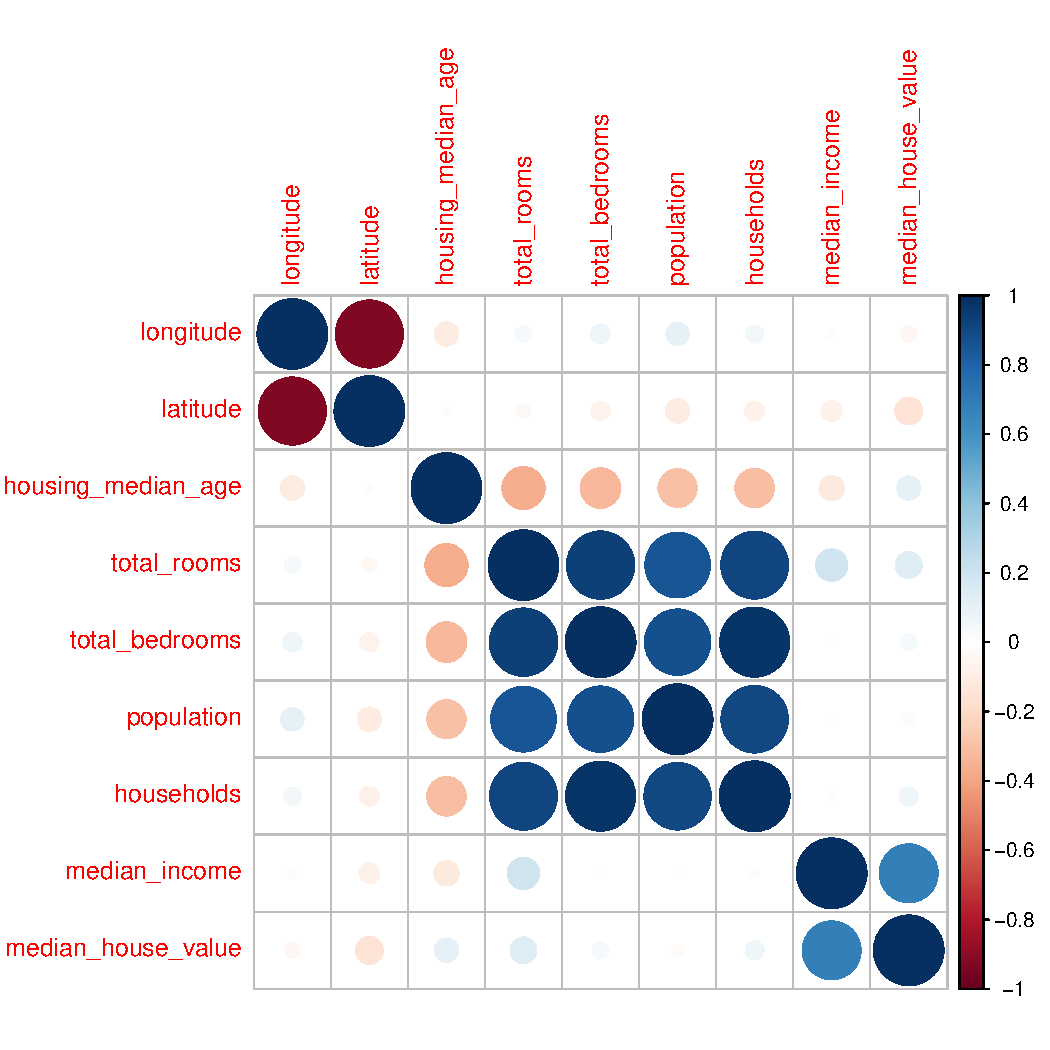
\includegraphics{hw5_files/figure-pdf/unnamed-chunk-3-1.pdf}

}

\end{figure}

\begin{center}\rule{0.5\linewidth}{0.5pt}\end{center}

1.3 (5 points)

Split the data \texttt{df} into \texttt{df\_train} and
\texttt{df\_split} using \texttt{test\_ind} in the code below:

\begin{Shaded}
\begin{Highlighting}[]
\FunctionTok{set.seed}\NormalTok{(}\DecValTok{42}\NormalTok{)}
\NormalTok{test\_ind }\OtherTok{\textless{}{-}} \FunctionTok{sample}\NormalTok{(}
  \DecValTok{1}\SpecialCharTok{:}\FunctionTok{nrow}\NormalTok{(df), }
  \FunctionTok{floor}\NormalTok{( }\FunctionTok{nrow}\NormalTok{(df)}\SpecialCharTok{/}\DecValTok{10}\NormalTok{ ),}
  \AttributeTok{replace=}\ConstantTok{FALSE}
\NormalTok{)}

\NormalTok{df\_train }\OtherTok{\textless{}{-}}\NormalTok{ ... }\CommentTok{\# Insert your code here}
\NormalTok{df\_test  }\OtherTok{\textless{}{-}}\NormalTok{ ... }\CommentTok{\# Insert your code here}
\end{Highlighting}
\end{Shaded}

\begin{Shaded}
\begin{Highlighting}[]
\FunctionTok{set.seed}\NormalTok{(}\DecValTok{42}\NormalTok{)}
\NormalTok{test\_ind }\OtherTok{\textless{}{-}} \FunctionTok{sample}\NormalTok{(}
  \DecValTok{1}\SpecialCharTok{:}\FunctionTok{nrow}\NormalTok{(df),}
  \FunctionTok{floor}\NormalTok{( }\FunctionTok{nrow}\NormalTok{(df) }\SpecialCharTok{/} \DecValTok{10}\NormalTok{ ),}
  \AttributeTok{replace=}\ConstantTok{FALSE}
\NormalTok{)}

\NormalTok{df\_train }\OtherTok{\textless{}{-}}\NormalTok{ df[}\SpecialCharTok{{-}}\NormalTok{test\_ind, ]}
\NormalTok{df\_test }\OtherTok{\textless{}{-}}\NormalTok{ df[test\_ind, ]}
\end{Highlighting}
\end{Shaded}

\begin{center}\rule{0.5\linewidth}{0.5pt}\end{center}

1.4 (5 points)

Fit a linear regression model to predict the
\texttt{median\_house\_value} :

\begin{itemize}
\tightlist
\item
  \texttt{latitude}
\item
  \texttt{longitude}
\item
  \texttt{housing\_median\_age}
\item
  \texttt{total\_rooms}
\item
  \texttt{total\_bedrooms}
\item
  \texttt{population}
\item
  \texttt{median\_income}
\item
  \texttt{ocean\_proximity}
\end{itemize}

Interpret the coefficients and summarize your results.

\begin{Shaded}
\begin{Highlighting}[]
\FunctionTok{library}\NormalTok{(dplyr)}
\FunctionTok{library}\NormalTok{(tidyr)}
\FunctionTok{library}\NormalTok{(modelr)}
\end{Highlighting}
\end{Shaded}

\begin{verbatim}

Attaching package: 'modelr'
\end{verbatim}

\begin{verbatim}
The following object is masked from 'package:broom':

    bootstrap
\end{verbatim}

\begin{Shaded}
\begin{Highlighting}[]
\NormalTok{lm\_fit }\OtherTok{\textless{}{-}} \FunctionTok{lm}\NormalTok{(median\_house\_value }\SpecialCharTok{\textasciitilde{}}\NormalTok{ latitude }\SpecialCharTok{+}\NormalTok{ longitude }\SpecialCharTok{+}\NormalTok{ housing\_median\_age }\SpecialCharTok{+} 
\NormalTok{              total\_rooms }\SpecialCharTok{+}\NormalTok{ total\_bedrooms }\SpecialCharTok{+}\NormalTok{ population }\SpecialCharTok{+}\NormalTok{ median\_income }\SpecialCharTok{+} 
\NormalTok{              ocean\_proximity, }\AttributeTok{data =}\NormalTok{ df)}

\FunctionTok{summary}\NormalTok{(lm\_fit)}
\end{Highlighting}
\end{Shaded}

\begin{verbatim}

Call:
lm(formula = median_house_value ~ latitude + longitude + housing_median_age + 
    total_rooms + total_bedrooms + population + median_income + 
    ocean_proximity, data = df)

Residuals:
    Min      1Q  Median      3Q     Max 
-560372  -42613  -10349   28958  718550 

Coefficients:
                            Estimate Std. Error t value Pr(>|t|)    
(Intercept)               -2.356e+06  8.714e+04 -27.040  < 2e-16 ***
latitude                  -2.624e+04  9.992e+02 -26.265  < 2e-16 ***
longitude                 -2.776e+04  1.011e+03 -27.463  < 2e-16 ***
housing_median_age         1.082e+03  4.391e+01  24.649  < 2e-16 ***
total_rooms               -6.445e+00  7.914e-01  -8.144 4.04e-16 ***
total_bedrooms             1.378e+02  3.987e+00  34.565  < 2e-16 ***
population                -3.449e+01  9.420e-01 -36.617  < 2e-16 ***
median_income              3.943e+04  3.374e+02 116.878  < 2e-16 ***
ocean_proximityINLAND     -3.926e+04  1.746e+03 -22.486  < 2e-16 ***
ocean_proximityISLAND      1.480e+05  3.077e+04   4.811 1.51e-06 ***
ocean_proximityNEAR BAY   -4.102e+03  1.915e+03  -2.142   0.0322 *  
ocean_proximityNEAR OCEAN  4.058e+03  1.571e+03   2.583   0.0098 ** 
---
Signif. codes:  0 '***' 0.001 '**' 0.01 '*' 0.05 '.' 0.1 ' ' 1

Residual standard error: 68730 on 20421 degrees of freedom
Multiple R-squared:  0.6457,    Adjusted R-squared:  0.6455 
F-statistic:  3383 on 11 and 20421 DF,  p-value: < 2.2e-16
\end{verbatim}

\begin{center}\rule{0.5\linewidth}{0.5pt}\end{center}

1.5 (5 points)

Complete the \texttt{rmse} function for computing the Root Mean-Squared
Error between the true \texttt{y} and the predicted \texttt{yhat}, and
use it to compute the RMSE for the regression model on \texttt{df\_test}

\begin{Shaded}
\begin{Highlighting}[]
\CommentTok{\# define}
\NormalTok{rmse }\OtherTok{\textless{}{-}} \ControlFlowTok{function}\NormalTok{(y, yhat) \{}
  \FunctionTok{sqrt}\NormalTok{(}\FunctionTok{mean}\NormalTok{((y }\SpecialCharTok{{-}}\NormalTok{ yhat)}\SpecialCharTok{\^{}}\DecValTok{2}\NormalTok{))}
\NormalTok{\}}

\CommentTok{\# predict}
\NormalTok{lm\_predictions }\OtherTok{\textless{}{-}} \FunctionTok{predict}\NormalTok{(lm\_fit, }\AttributeTok{newdata =}\NormalTok{ df\_test)}

\CommentTok{\# calculate}
\NormalTok{rmse\_value }\OtherTok{\textless{}{-}} \FunctionTok{rmse}\NormalTok{(df\_test}\SpecialCharTok{$}\NormalTok{median\_house\_value, lm\_predictions)}

\CommentTok{\# output}
\NormalTok{rmse\_value}
\end{Highlighting}
\end{Shaded}

\begin{verbatim}
[1] 68272.54
\end{verbatim}

1.6 (5 points)

Fit a decision tree model to predict the \texttt{median\_house\_value}
using the same predictors as in 1.4. Use the \texttt{rpart()} function.

Visualize the decision tree using the \texttt{rpart.plot()} function.

Report the root mean squared error on the test set.

\begin{Shaded}
\begin{Highlighting}[]
\FunctionTok{library}\NormalTok{(rpart)}
\FunctionTok{library}\NormalTok{(rpart.plot)}

\NormalTok{rpart\_fit }\OtherTok{\textless{}{-}} \FunctionTok{rpart}\NormalTok{(median\_house\_value }\SpecialCharTok{\textasciitilde{}}\NormalTok{ latitude }\SpecialCharTok{+}\NormalTok{ longitude }\SpecialCharTok{+}\NormalTok{ housing\_median\_age }\SpecialCharTok{+} 
\NormalTok{                   total\_rooms }\SpecialCharTok{+}\NormalTok{ total\_bedrooms }\SpecialCharTok{+}\NormalTok{ population }\SpecialCharTok{+}\NormalTok{ median\_income }\SpecialCharTok{+} 
\NormalTok{                   ocean\_proximity, }\AttributeTok{data =}\NormalTok{ df\_train)}

\NormalTok{rpart\_predictions }\OtherTok{\textless{}{-}} \FunctionTok{predict}\NormalTok{(rpart\_fit, }\AttributeTok{newdata =}\NormalTok{ df\_test)}

\FunctionTok{rpart.plot}\NormalTok{(rpart\_fit)}
\end{Highlighting}
\end{Shaded}

\begin{figure}[H]

{\centering 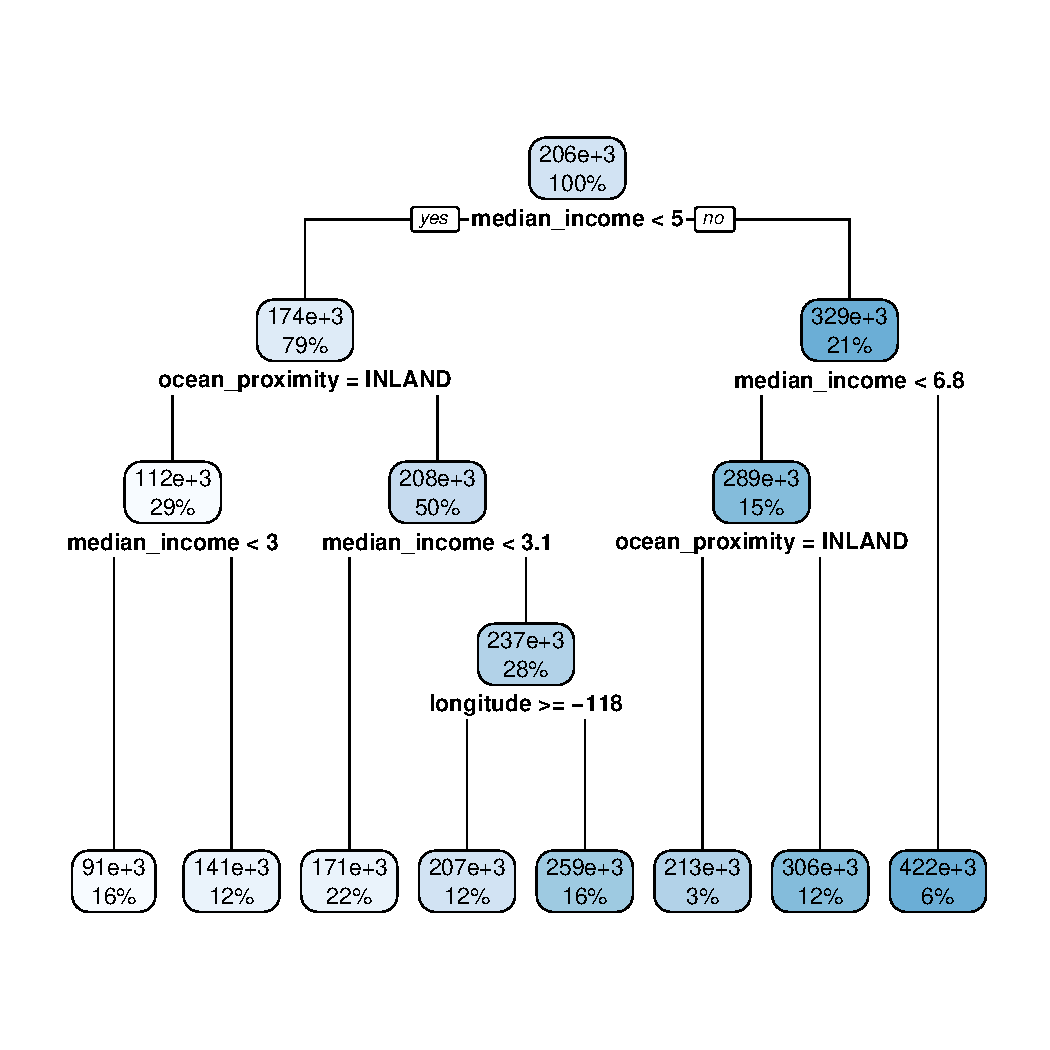
\includegraphics{hw5_files/figure-pdf/unnamed-chunk-7-1.pdf}

}

\end{figure}

\begin{Shaded}
\begin{Highlighting}[]
\NormalTok{rmse\_rpart }\OtherTok{\textless{}{-}} \FunctionTok{sqrt}\NormalTok{(}\FunctionTok{mean}\NormalTok{((df\_test}\SpecialCharTok{$}\NormalTok{median\_house\_value }\SpecialCharTok{{-}}\NormalTok{ rpart\_predictions)}\SpecialCharTok{\^{}}\DecValTok{2}\NormalTok{))}
\NormalTok{rmse\_rpart}
\end{Highlighting}
\end{Shaded}

\begin{verbatim}
[1] 75876.87
\end{verbatim}

\begin{center}\rule{0.5\linewidth}{0.5pt}\end{center}

1.7 (5 points)

Fit a support vector machine model to predict the
\texttt{median\_house\_value} using the same predictors as in 1.4. Use
the \texttt{svm()} function and use any kernel of your choice. Report
the root mean squared error on the test set.

\begin{Shaded}
\begin{Highlighting}[]
\FunctionTok{library}\NormalTok{(e1071)}

\NormalTok{svm\_fit }\OtherTok{\textless{}{-}} \FunctionTok{svm}\NormalTok{(median\_house\_value }\SpecialCharTok{\textasciitilde{}}\NormalTok{ latitude }\SpecialCharTok{+}\NormalTok{ longitude }\SpecialCharTok{+}\NormalTok{ housing\_median\_age }\SpecialCharTok{+} 
\NormalTok{               total\_rooms }\SpecialCharTok{+}\NormalTok{ total\_bedrooms }\SpecialCharTok{+}\NormalTok{ population }\SpecialCharTok{+}\NormalTok{ median\_income }\SpecialCharTok{+} 
\NormalTok{               ocean\_proximity, }\AttributeTok{data =}\NormalTok{ df\_train, }\AttributeTok{kernel =} \StringTok{"radial"}\NormalTok{) }

\NormalTok{svm\_predictions }\OtherTok{\textless{}{-}} \FunctionTok{predict}\NormalTok{(svm\_fit, }\AttributeTok{newdata =}\NormalTok{ df\_test)}

\NormalTok{rmse\_svm }\OtherTok{\textless{}{-}} \FunctionTok{sqrt}\NormalTok{(}\FunctionTok{mean}\NormalTok{((df\_test}\SpecialCharTok{$}\NormalTok{median\_house\_value }\SpecialCharTok{{-}}\NormalTok{ svm\_predictions)}\SpecialCharTok{\^{}}\DecValTok{2}\NormalTok{))}
\NormalTok{rmse\_svm}
\end{Highlighting}
\end{Shaded}

\begin{verbatim}
[1] 56678.84
\end{verbatim}

\begin{center}\rule{0.5\linewidth}{0.5pt}\end{center}

1.8 (25 points)

Initialize a neural network model architecture:

\begin{Shaded}
\begin{Highlighting}[]
\FunctionTok{library}\NormalTok{(torch)}
\FunctionTok{library}\NormalTok{(luz)}
\FunctionTok{library}\NormalTok{(tidyverse)}
\end{Highlighting}
\end{Shaded}

\begin{verbatim}
-- Attaching core tidyverse packages ------------------------ tidyverse 2.0.0 --
v forcats   1.0.0     v stringr   1.5.1
v lubridate 1.9.3     
-- Conflicts ------------------------------------------ tidyverse_conflicts() --
x modelr::bootstrap()   masks broom::bootstrap()
x magrittr::extract()   masks tidyr::extract()
x dplyr::filter()       masks stats::filter()
x dplyr::lag()          masks stats::lag()
x caret::lift()         masks purrr::lift()
x magrittr::set_names() masks purrr::set_names()
i Use the conflicted package (<http://conflicted.r-lib.org/>) to force all conflicts to become errors
\end{verbatim}

\begin{Shaded}
\begin{Highlighting}[]
\NormalTok{NNet }\OtherTok{\textless{}{-}} \FunctionTok{nn\_module}\NormalTok{(}
  \AttributeTok{initialize =} \ControlFlowTok{function}\NormalTok{(p, q1, q2, q3) \{}
\NormalTok{    self}\SpecialCharTok{$}\NormalTok{net }\OtherTok{\textless{}{-}} \FunctionTok{nn\_sequential}\NormalTok{(}
      \FunctionTok{nn\_linear}\NormalTok{(p, q1), }\FunctionTok{nn\_relu}\NormalTok{(),}
      \FunctionTok{nn\_linear}\NormalTok{(q1, q2), }\FunctionTok{nn\_relu}\NormalTok{(),}
      \FunctionTok{nn\_linear}\NormalTok{(q2, q3), }\FunctionTok{nn\_relu}\NormalTok{(),}
      \FunctionTok{nn\_linear}\NormalTok{(q3, }\DecValTok{1}\NormalTok{)}
\NormalTok{    )}
\NormalTok{  \},}
  \AttributeTok{forward =} \ControlFlowTok{function}\NormalTok{(x) \{}
\NormalTok{    self}\SpecialCharTok{$}\FunctionTok{net}\NormalTok{(x)}
\NormalTok{  \}}
\NormalTok{)}
\end{Highlighting}
\end{Shaded}

Fit a neural network model to predict the \texttt{median\_house\_value}
using the same predictors as in 1.4. Use the \texttt{model.matrix}
function to create the covariate matrix and \texttt{luz} package for
fitting the network with \(32, 16, 8\) nodes in each of the three hidden
layers.

\begin{Shaded}
\begin{Highlighting}[]
\NormalTok{nnet\_fit }\OtherTok{\textless{}{-}}\NormalTok{ NNet }\SpecialCharTok{\%\textgreater{}\%} 
  \FunctionTok{setup}\NormalTok{(}
\NormalTok{    ... }\CommentTok{\# Insert your code here}
\NormalTok{  ) }\SpecialCharTok{\%\textgreater{}\%}
  \FunctionTok{set\_hparams}\NormalTok{(}
\NormalTok{    ... }\CommentTok{\# Insert your code here}
\NormalTok{  ) }\SpecialCharTok{\%\textgreater{}\%}
  \FunctionTok{set\_opt\_params}\NormalTok{(}
\NormalTok{    ... }\CommentTok{\# Insert your code here}
\NormalTok{  ) }\SpecialCharTok{\%\textgreater{}\%}
  \FunctionTok{fit}\NormalTok{(}
\NormalTok{    ... }\CommentTok{\# Insert your code here}
    \AttributeTok{dataloader\_options =}\NormalTok{ ... }\CommentTok{\# Insert your code here}
    \AttributeTok{verbose =} \ConstantTok{FALSE} \CommentTok{\# Change to TRUE while tuning. But, set to FALSE before submitting}

\NormalTok{  )}
\end{Highlighting}
\end{Shaded}

\begin{Shaded}
\begin{Highlighting}[]
\NormalTok{X\_train }\OtherTok{\textless{}{-}} \FunctionTok{model.matrix}\NormalTok{(}\SpecialCharTok{\textasciitilde{}}\NormalTok{ . }\SpecialCharTok{{-}}\NormalTok{ median\_house\_value }\SpecialCharTok{{-}}\NormalTok{ households, }\AttributeTok{data =}\NormalTok{ df\_train)}
\NormalTok{y\_train }\OtherTok{\textless{}{-}} \FunctionTok{as.matrix}\NormalTok{(df\_train}\SpecialCharTok{$}\NormalTok{median\_house\_value)}


\NormalTok{nnet\_fit }\OtherTok{\textless{}{-}}\NormalTok{ NNet }\SpecialCharTok{\%\textgreater{}\%} 
  \FunctionTok{setup}\NormalTok{(}
    \AttributeTok{loss =} \FunctionTok{nn\_mse\_loss}\NormalTok{(),}
    \AttributeTok{optimizer =}\NormalTok{ optim\_adam}
\NormalTok{  ) }\SpecialCharTok{\%\textgreater{}\%}
  \FunctionTok{set\_hparams}\NormalTok{(}
    \AttributeTok{p =} \FunctionTok{ncol}\NormalTok{(X\_train),}
    \AttributeTok{q1 =} \DecValTok{32}\NormalTok{,}
    \AttributeTok{q2 =} \DecValTok{16}\NormalTok{,}
    \AttributeTok{q3 =} \DecValTok{8}
\NormalTok{  ) }\SpecialCharTok{\%\textgreater{}\%} 
  \FunctionTok{set\_opt\_hparams}\NormalTok{(}\AttributeTok{lr =} \FloatTok{0.01}\NormalTok{) }\SpecialCharTok{\%\textgreater{}\%}
  \FunctionTok{fit}\NormalTok{(}
    \FunctionTok{list}\NormalTok{(X\_train, y\_train),}
    \AttributeTok{epochs =} \DecValTok{40}\NormalTok{,}
    \AttributeTok{dataloader\_options =} \FunctionTok{list}\NormalTok{(}\AttributeTok{batch\_size =} \DecValTok{64}\NormalTok{),}
    \AttributeTok{verbose =} \ConstantTok{FALSE}\NormalTok{, }\CommentTok{\# Change to TRUE while tuning. But, set to FALSE before submitting}
    \AttributeTok{valid\_data =} \FloatTok{0.2}
\NormalTok{  )}
\end{Highlighting}
\end{Shaded}

Plot the results of the training and validation loss and accuracy.

\begin{Shaded}
\begin{Highlighting}[]
\FunctionTok{plot}\NormalTok{(nnet\_fit)}
\end{Highlighting}
\end{Shaded}

\begin{figure}[H]

{\centering 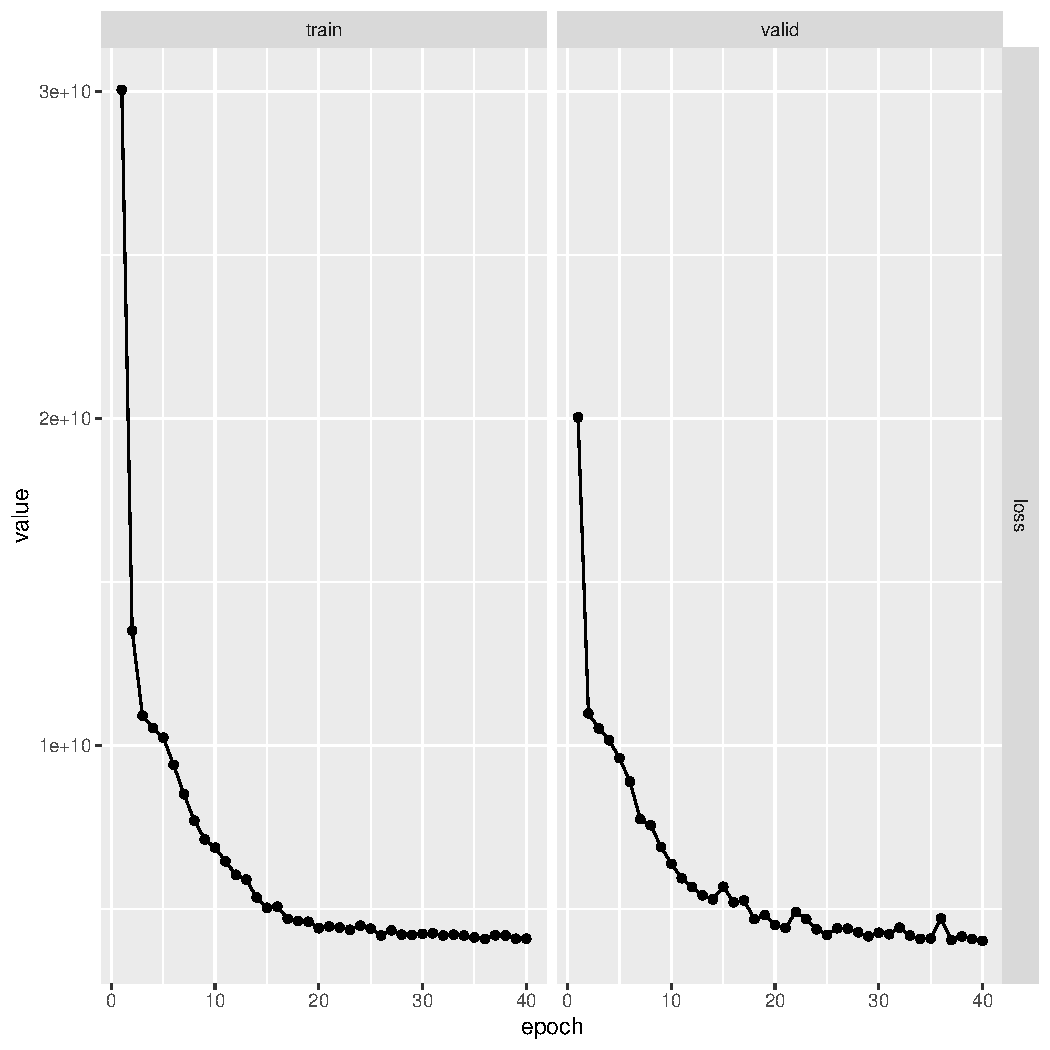
\includegraphics{hw5_files/figure-pdf/unnamed-chunk-11-1.pdf}

}

\end{figure}

Report the root mean squared error on the test set.

\begin{Shaded}
\begin{Highlighting}[]
\NormalTok{nnet\_predictions }\OtherTok{\textless{}{-}}\NormalTok{ ... }\CommentTok{\# Insert your code here}
\end{Highlighting}
\end{Shaded}

\begin{Shaded}
\begin{Highlighting}[]
\NormalTok{X\_test }\OtherTok{\textless{}{-}} \FunctionTok{model.matrix}\NormalTok{(}\SpecialCharTok{\textasciitilde{}}\NormalTok{ . }\SpecialCharTok{{-}}\NormalTok{ median\_house\_value }\SpecialCharTok{{-}}\NormalTok{ households, }\AttributeTok{data =}\NormalTok{ df\_test)}
\CommentTok{\#}
\NormalTok{nnet\_predictions }\OtherTok{\textless{}{-}}\NormalTok{ nnet\_fit }\SpecialCharTok{\%\textgreater{}\%} \FunctionTok{predict}\NormalTok{(X\_test)}
\NormalTok{rmse\_nn }\OtherTok{\textless{}{-}} \FunctionTok{rmse}\NormalTok{(}\FunctionTok{as\_array}\NormalTok{(nnet\_predictions), df\_test}\SpecialCharTok{$}\NormalTok{median\_house\_value)}
\FunctionTok{cat}\NormalTok{(}\StringTok{"The RMSE of Neural Network is: "}\NormalTok{, rmse\_nn)}
\end{Highlighting}
\end{Shaded}

\begin{verbatim}
The RMSE of Neural Network is:  63372.72
\end{verbatim}

\begin{tcolorbox}[enhanced jigsaw, bottomtitle=1mm, rightrule=.15mm, left=2mm, colback=white, opacityback=0, bottomrule=.15mm, titlerule=0mm, toprule=.15mm, colframe=quarto-callout-warning-color-frame, arc=.35mm, colbacktitle=quarto-callout-warning-color!10!white, breakable, leftrule=.75mm, coltitle=black, title=\textcolor{quarto-callout-warning-color}{\faExclamationTriangle}\hspace{0.5em}{Warning}, opacitybacktitle=0.6, toptitle=1mm]

Remember to use the \texttt{as\_array()} function to convert the
predictions to a vector of numbers before computing the RMSE with
\texttt{rmse()}

\end{tcolorbox}

\begin{center}\rule{0.5\linewidth}{0.5pt}\end{center}

1.9 (5 points)

Summarize your results in a table comparing the RMSE for the different
models. Which model performed best? Why do you think that is?

\begin{Shaded}
\begin{Highlighting}[]
\NormalTok{... }\CommentTok{\# Insert your code here}
\end{Highlighting}
\end{Shaded}

\begin{Shaded}
\begin{Highlighting}[]
\NormalTok{rmse\_performance }\OtherTok{\textless{}{-}} \FunctionTok{tibble}\NormalTok{(}\StringTok{\textasciigrave{}}\AttributeTok{Foreccasting model}\StringTok{\textasciigrave{}} \OtherTok{=} \FunctionTok{c}\NormalTok{(}\StringTok{"Linear regression"}\NormalTok{, }\StringTok{"Decision Tree"}\NormalTok{,}
                                                    \StringTok{"SVM"}\NormalTok{, }\StringTok{"Neural Network"}\NormalTok{),}
                           \AttributeTok{RMSE =} \FunctionTok{c}\NormalTok{(rmse\_value, rmse\_rpart, rmse\_svm, rmse\_nn))}
\NormalTok{rmse\_performance}
\end{Highlighting}
\end{Shaded}

\begin{verbatim}
# A tibble: 4 x 2
  `Foreccasting model`   RMSE
  <chr>                 <dbl>
1 Linear regression    68273.
2 Decision Tree        75877.
3 SVM                  56679.
4 Neural Network       63373.
\end{verbatim}

---

\hypertarget{question-2}{%
\subsection{Question 2}\label{question-2}}

\begin{tcolorbox}[enhanced jigsaw, bottomtitle=1mm, rightrule=.15mm, left=2mm, colback=white, opacityback=0, bottomrule=.15mm, titlerule=0mm, toprule=.15mm, colframe=quarto-callout-tip-color-frame, arc=.35mm, colbacktitle=quarto-callout-tip-color!10!white, breakable, leftrule=.75mm, coltitle=black, title=\textcolor{quarto-callout-tip-color}{\faLightbulb}\hspace{0.5em}{50 points}, opacitybacktitle=0.6, toptitle=1mm]

Spam email classification

\end{tcolorbox}

The \texttt{data} folder contains the \texttt{spam.csv} dataset. This
dataset contains features extracted from a collection of spam and
non-spam emails. The objective is to classify the emails as spam or
non-spam.

\begin{center}\rule{0.5\linewidth}{0.5pt}\end{center}

2.1 (2.5 points)

Read the data file as a tibble in R. Preprocess the data such that:

\begin{enumerate}
\def\labelenumi{\arabic{enumi}.}
\tightlist
\item
  the variables are of the right data type, e.g., categorical variables
  are encoded as factors
\item
  all column names to lower case for consistency
\item
  Any observations with missing values are dropped
\end{enumerate}

\begin{Shaded}
\begin{Highlighting}[]
\NormalTok{df }\OtherTok{\textless{}{-}}\NormalTok{ ... }\CommentTok{\# Insert your code here}
\end{Highlighting}
\end{Shaded}

\begin{Shaded}
\begin{Highlighting}[]
\FunctionTok{library}\NormalTok{(tidyverse)}

\CommentTok{\# 读取数据}
\NormalTok{path }\OtherTok{\textless{}{-}} \StringTok{"data/spambase.csv"}
\NormalTok{df }\OtherTok{\textless{}{-}} \FunctionTok{read\_csv}\NormalTok{(path) }\SpecialCharTok{\%\textgreater{}\%}
  \FunctionTok{mutate}\NormalTok{(}\FunctionTok{across}\NormalTok{(is.character, as.factor)) }\SpecialCharTok{\%\textgreater{}\%} \CommentTok{\# 将所有变量转换为因子类型}
  \FunctionTok{rename\_with}\NormalTok{(tolower) }\SpecialCharTok{\%\textgreater{}\%} \CommentTok{\# 列名转换为小写}
  \FunctionTok{drop\_na}\NormalTok{() }\CommentTok{\# 删除包含缺失值的观察值}
\end{Highlighting}
\end{Shaded}

\begin{verbatim}
Rows: 4601 Columns: 58
-- Column specification --------------------------------------------------------
Delimiter: ","
dbl (58): word_freq_1, word_freq_2, word_freq_3, word_freq_4, word_freq_5, w...

i Use `spec()` to retrieve the full column specification for this data.
i Specify the column types or set `show_col_types = FALSE` to quiet this message.
\end{verbatim}

\begin{verbatim}
Warning: There was 1 warning in `mutate()`.
i In argument: `across(is.character, as.factor)`.
Caused by warning:
! Use of bare predicate functions was deprecated in tidyselect 1.1.0.
i Please use wrap predicates in `where()` instead.
  # Was:
  data %>% select(is.character)

  # Now:
  data %>% select(where(is.character))
\end{verbatim}

\begin{Shaded}
\begin{Highlighting}[]
\NormalTok{df}\SpecialCharTok{$}\NormalTok{spam }\OtherTok{\textless{}{-}} \FunctionTok{factor}\NormalTok{(df}\SpecialCharTok{$}\NormalTok{spam)}

\CommentTok{\# 显示处理后的数据}
\FunctionTok{head}\NormalTok{(df)}
\end{Highlighting}
\end{Shaded}

\begin{verbatim}
# A tibble: 6 x 58
  word_freq_1 word_freq_2 word_freq_3 word_freq_4 word_freq_5 word_freq_6
        <dbl>       <dbl>       <dbl>       <dbl>       <dbl>       <dbl>
1        0           0.64        0.64           0        0.32        0   
2        0.21        0.28        0.5            0        0.14        0.28
3        0.06        0           0.71           0        1.23        0.19
4        0           0           0              0        0.63        0   
5        0           0           0              0        0.63        0   
6        0           0           0              0        1.85        0   
# i 52 more variables: word_freq_7 <dbl>, word_freq_8 <dbl>, word_freq_9 <dbl>,
#   word_freq_10 <dbl>, word_freq_11 <dbl>, word_freq_12 <dbl>,
#   word_freq_13 <dbl>, word_freq_14 <dbl>, word_freq_15 <dbl>,
#   word_freq_16 <dbl>, word_freq_17 <dbl>, word_freq_18 <dbl>,
#   word_freq_19 <dbl>, word_freq_20 <dbl>, word_freq_21 <dbl>,
#   word_freq_22 <dbl>, word_freq_23 <dbl>, word_freq_24 <dbl>,
#   word_freq_25 <dbl>, word_freq_26 <dbl>, word_freq_27 <dbl>, ...
\end{verbatim}

\begin{Shaded}
\begin{Highlighting}[]
\CommentTok{\#}
\end{Highlighting}
\end{Shaded}

\begin{center}\rule{0.5\linewidth}{0.5pt}\end{center}

2.2 (2.5 points)

Split the data \texttt{df} into \texttt{df\_train} and
\texttt{df\_split} using \texttt{test\_ind} in the code below:

\begin{Shaded}
\begin{Highlighting}[]
\FunctionTok{set.seed}\NormalTok{(}\DecValTok{42}\NormalTok{)}
\NormalTok{test\_ind }\OtherTok{\textless{}{-}} \FunctionTok{sample}\NormalTok{(}
  \DecValTok{1}\SpecialCharTok{:}\FunctionTok{nrow}\NormalTok{(df), }
  \FunctionTok{floor}\NormalTok{( }\FunctionTok{nrow}\NormalTok{(df)}\SpecialCharTok{/}\DecValTok{10}\NormalTok{ ),}
  \AttributeTok{replace=}\ConstantTok{FALSE}
\NormalTok{)}

\NormalTok{df\_train2 }\OtherTok{\textless{}{-}}\NormalTok{ df[}\SpecialCharTok{{-}}\NormalTok{test\_ind, ]}
\NormalTok{df\_test2 }\OtherTok{\textless{}{-}}\NormalTok{ df[test\_ind, ]}
\end{Highlighting}
\end{Shaded}

Complete the \texttt{overview} function which returns a data frame with
the following columns: \texttt{accuracy}, \texttt{error},
\texttt{false\ positive\ rate}, \texttt{true\ positive\ rate}, between
the true \texttt{true\_class} and the predicted \texttt{pred\_class} for
any classification model.

\begin{Shaded}
\begin{Highlighting}[]
\NormalTok{overview }\OtherTok{\textless{}{-}} \ControlFlowTok{function}\NormalTok{(pred\_class, true\_class) \{}
\NormalTok{  accuracy }\OtherTok{\textless{}{-}} \FunctionTok{mean}\NormalTok{(pred\_class }\SpecialCharTok{==}\NormalTok{ true\_class)}
\NormalTok{  error }\OtherTok{\textless{}{-}} \FunctionTok{mean}\NormalTok{(pred\_class }\SpecialCharTok{!=}\NormalTok{ true\_class)}
\NormalTok{  true\_positives }\OtherTok{\textless{}{-}} \FunctionTok{sum}\NormalTok{(true\_class }\SpecialCharTok{==} \DecValTok{1} \SpecialCharTok{\&}\NormalTok{ pred\_class }\SpecialCharTok{==} \DecValTok{1}\NormalTok{)}
\NormalTok{  true\_negatives }\OtherTok{\textless{}{-}} \FunctionTok{sum}\NormalTok{(true\_class }\SpecialCharTok{==} \DecValTok{0} \SpecialCharTok{\&}\NormalTok{ pred\_class }\SpecialCharTok{==} \DecValTok{0}\NormalTok{)}
\NormalTok{  false\_positives }\OtherTok{\textless{}{-}} \FunctionTok{sum}\NormalTok{(true\_class }\SpecialCharTok{==} \DecValTok{0} \SpecialCharTok{\&}\NormalTok{ pred\_class }\SpecialCharTok{==} \DecValTok{1}\NormalTok{)}
\NormalTok{  false\_negatives }\OtherTok{\textless{}{-}} \FunctionTok{sum}\NormalTok{(true\_class }\SpecialCharTok{==} \DecValTok{1} \SpecialCharTok{\&}\NormalTok{ pred\_class }\SpecialCharTok{==} \DecValTok{0}\NormalTok{)}
\NormalTok{  true\_positive\_rate }\OtherTok{\textless{}{-}}\NormalTok{ true\_positives }\SpecialCharTok{/}\NormalTok{ (true\_positives }\SpecialCharTok{+}\NormalTok{ false\_negatives)}
\NormalTok{  false\_positive\_rate }\OtherTok{\textless{}{-}}\NormalTok{ false\_positives }\SpecialCharTok{/}\NormalTok{ (true\_negatives }\SpecialCharTok{+}\NormalTok{ false\_positives)}
  
  \FunctionTok{return}\NormalTok{(}
    \FunctionTok{data.frame}\NormalTok{(}
      \AttributeTok{accuracy =}\NormalTok{ accuracy,}
      \AttributeTok{error =}\NormalTok{ error,}
      \AttributeTok{true\_positive\_rate =}\NormalTok{ true\_positive\_rate,}
      \AttributeTok{false\_positive\_rate =}\NormalTok{ false\_positive\_rate}
\NormalTok{    )}
\NormalTok{  )}
\NormalTok{\}}
\end{Highlighting}
\end{Shaded}

\begin{center}\rule{0.5\linewidth}{0.5pt}\end{center}

2.3 (5 points)

Fit a logistic regression model to predict the \texttt{spam} variable
using the remaining predictors. Report the prediction accuracy on the
test set.

\begin{Shaded}
\begin{Highlighting}[]
\NormalTok{glm\_fit }\OtherTok{\textless{}{-}}\NormalTok{ ... }\CommentTok{\# Insert your code here}
\NormalTok{glm\_classes }\OtherTok{\textless{}{-}}\NormalTok{ ... }\CommentTok{\# Insert your code here}
\end{Highlighting}
\end{Shaded}

\begin{Shaded}
\begin{Highlighting}[]
\NormalTok{glm\_fit }\OtherTok{\textless{}{-}} \FunctionTok{glm}\NormalTok{(spam }\SpecialCharTok{\textasciitilde{}}\NormalTok{ ., }\AttributeTok{data =}\NormalTok{ df\_train2, }\AttributeTok{family =} \StringTok{"binomial"}\NormalTok{)}
\end{Highlighting}
\end{Shaded}

\begin{verbatim}
Warning: glm.fit: fitted probabilities numerically 0 or 1 occurred
\end{verbatim}

\begin{Shaded}
\begin{Highlighting}[]
\NormalTok{glm\_pred }\OtherTok{\textless{}{-}} \FunctionTok{predict}\NormalTok{(glm\_fit, df\_test2, }\AttributeTok{type =} \StringTok{"response"}\NormalTok{)}
\NormalTok{glm\_classes }\OtherTok{\textless{}{-}} \FunctionTok{ifelse}\NormalTok{(glm\_pred }\SpecialCharTok{\textgreater{}} \FloatTok{0.5}\NormalTok{, }\DecValTok{1}\NormalTok{, }\DecValTok{0}\NormalTok{)}
\NormalTok{glm\_overview }\OtherTok{\textless{}{-}} \FunctionTok{overview}\NormalTok{(glm\_classes, df\_test2}\SpecialCharTok{$}\NormalTok{spam)}
\NormalTok{glm\_overview}
\end{Highlighting}
\end{Shaded}

\begin{verbatim}
  accuracy      error true_positive_rate false_positive_rate
1 0.923913 0.07608696          0.8670213          0.03676471
\end{verbatim}

\begin{center}\rule{0.5\linewidth}{0.5pt}\end{center}

2.4 (5 points)

Fit a decision tree model to predict the \texttt{spam} variable using
the remaining predictors. Use the \texttt{rpart()} function and set the
\texttt{method} argument to \texttt{"class"}.

Visualize the decision tree using the \texttt{rpart.plot()} function.

Report the prediction accuracy on the test set.

\begin{Shaded}
\begin{Highlighting}[]
\FunctionTok{library}\NormalTok{(rpart)}
\NormalTok{rpart\_model }\OtherTok{\textless{}{-}} \FunctionTok{rpart}\NormalTok{(spam }\SpecialCharTok{\textasciitilde{}}\NormalTok{ ., }\AttributeTok{data=}\NormalTok{df\_train2, }\AttributeTok{method=}\StringTok{"class"}\NormalTok{)}
\FunctionTok{library}\NormalTok{(rpart.plot)}
\FunctionTok{rpart.plot}\NormalTok{(rpart\_model)}
\end{Highlighting}
\end{Shaded}

\begin{figure}[H]

{\centering 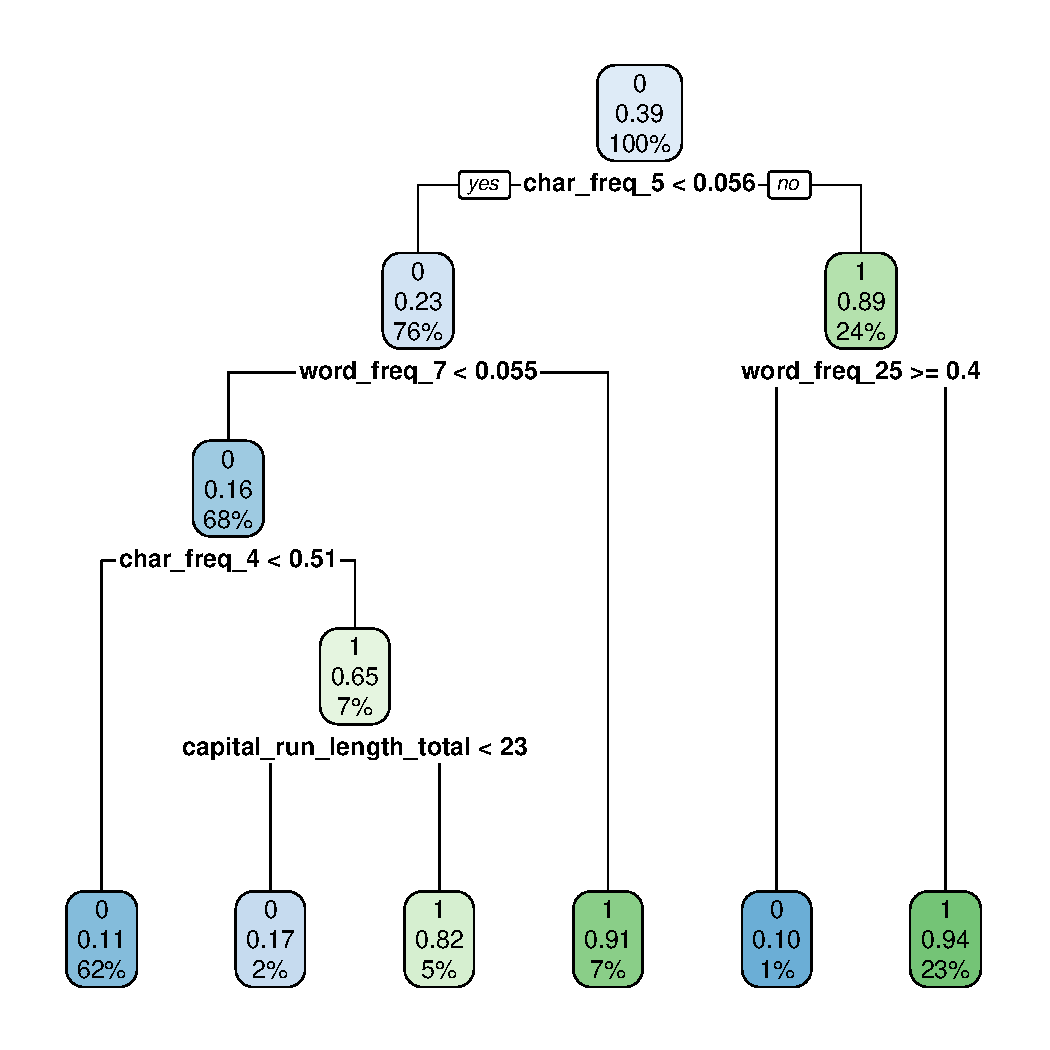
\includegraphics{hw5_files/figure-pdf/unnamed-chunk-18-1.pdf}

}

\end{figure}

\begin{Shaded}
\begin{Highlighting}[]
\NormalTok{predictions }\OtherTok{\textless{}{-}} \FunctionTok{predict}\NormalTok{(rpart\_model, }\AttributeTok{newdata=}\NormalTok{df\_test2, }\AttributeTok{type=}\StringTok{"class"}\NormalTok{)}
\NormalTok{rpart\_overview }\OtherTok{\textless{}{-}} \FunctionTok{overview}\NormalTok{(predictions, df\_test2}\SpecialCharTok{$}\NormalTok{spam)}
\NormalTok{rpart\_overview}
\end{Highlighting}
\end{Shaded}

\begin{verbatim}
   accuracy     error true_positive_rate false_positive_rate
1 0.8782609 0.1217391           0.787234          0.05882353
\end{verbatim}

\begin{center}\rule{0.5\linewidth}{0.5pt}\end{center}

2.5 (5 points)

Fit a support vector machine model to predict the \texttt{spam} variable
using the remaining predictors. Use the \texttt{svm()} function and use
any kernel of your choice. Remember to set the \texttt{type} argument to
\texttt{"C-classification"} \textbf{if you haven't} already converted
\texttt{spam} to be of type \texttt{factor}.

\begin{Shaded}
\begin{Highlighting}[]
\NormalTok{svm\_fit }\OtherTok{\textless{}{-}}\NormalTok{ ... }\CommentTok{\# Insert your code here}
\end{Highlighting}
\end{Shaded}

\begin{Shaded}
\begin{Highlighting}[]
\FunctionTok{library}\NormalTok{(e1071)}

\NormalTok{svm\_fit }\OtherTok{\textless{}{-}} \FunctionTok{svm}\NormalTok{(spam }\SpecialCharTok{\textasciitilde{}}\NormalTok{ ., }\AttributeTok{data=}\NormalTok{df\_train2, }\AttributeTok{type=}\StringTok{"C{-}classification"}\NormalTok{, }\AttributeTok{kernel=}\StringTok{"radial"}\NormalTok{)}
\end{Highlighting}
\end{Shaded}

Report the prediction accuracy on the test set.

\begin{Shaded}
\begin{Highlighting}[]
\NormalTok{svm\_classes }\OtherTok{\textless{}{-}}\NormalTok{ ... }\CommentTok{\# Insert your code here}
\end{Highlighting}
\end{Shaded}

\begin{Shaded}
\begin{Highlighting}[]
\NormalTok{svm\_predictions }\OtherTok{\textless{}{-}} \FunctionTok{predict}\NormalTok{(svm\_fit, }\AttributeTok{newdata=}\NormalTok{df\_test2)}
\NormalTok{svm\_overview }\OtherTok{\textless{}{-}} \FunctionTok{overview}\NormalTok{(svm\_predictions, df\_test2}\SpecialCharTok{$}\NormalTok{spam)}
\NormalTok{svm\_overview}
\end{Highlighting}
\end{Shaded}

\begin{verbatim}
  accuracy      error true_positive_rate false_positive_rate
1 0.923913 0.07608696          0.8776596          0.04411765
\end{verbatim}

\begin{center}\rule{0.5\linewidth}{0.5pt}\end{center}

2.6 (25 points)

Using the same neural network architecture as in 1.9, fit a neural
network model to predict the \texttt{spam} variable using the remaining
predictors.

\begin{tcolorbox}[enhanced jigsaw, bottomtitle=1mm, rightrule=.15mm, left=2mm, colback=white, opacityback=0, bottomrule=.15mm, titlerule=0mm, toprule=.15mm, colframe=quarto-callout-warning-color-frame, arc=.35mm, colbacktitle=quarto-callout-warning-color!10!white, breakable, leftrule=.75mm, coltitle=black, title=\textcolor{quarto-callout-warning-color}{\faExclamationTriangle}\hspace{0.5em}{Classification vs.~Regression}, opacitybacktitle=0.6, toptitle=1mm]

Note that the neural network in \textbf{Q 1.9} was a regression model.
You will need to modify the neural network architecture to be a
classification model by changing the output layer to have a single node
with a sigmoid activation function.

\end{tcolorbox}

Use the \texttt{model.matrix} function to create the covariate matrix
and \texttt{luz} package for fitting the network with \(32, 16, 8\)
nodes in each of the three hidden layers.

\begin{Shaded}
\begin{Highlighting}[]
\FunctionTok{library}\NormalTok{(torch)}
\FunctionTok{library}\NormalTok{(luz)}

\NormalTok{NNet\_binary }\OtherTok{\textless{}{-}} \FunctionTok{nn\_module}\NormalTok{(}
  \AttributeTok{initialize =} \ControlFlowTok{function}\NormalTok{(p, q1, q2, q3) \{}
\NormalTok{    self}\SpecialCharTok{$}\NormalTok{net }\OtherTok{\textless{}{-}} \FunctionTok{nn\_sequential}\NormalTok{(}
      \FunctionTok{nn\_linear}\NormalTok{(p, q1), }\FunctionTok{nn\_relu}\NormalTok{(),}
      \FunctionTok{nn\_linear}\NormalTok{(q1, q2), }\FunctionTok{nn\_relu}\NormalTok{(),}
      \FunctionTok{nn\_linear}\NormalTok{(q2, q3), }\FunctionTok{nn\_relu}\NormalTok{(),}
      \FunctionTok{nn\_linear}\NormalTok{(q3, }\DecValTok{1}\NormalTok{)}
\NormalTok{    )}
\NormalTok{    self}\SpecialCharTok{$}\NormalTok{activation }\OtherTok{\textless{}{-}} \FunctionTok{nn\_sigmoid}\NormalTok{()}
\NormalTok{  \},}
  \AttributeTok{forward =} \ControlFlowTok{function}\NormalTok{(x) \{}
\NormalTok{    self}\SpecialCharTok{$}\FunctionTok{net}\NormalTok{(x) }\SpecialCharTok{\%\textgreater{}\%}\NormalTok{ self}\SpecialCharTok{$}\FunctionTok{activation}\NormalTok{()}
\NormalTok{  \}}
\NormalTok{)}
\end{Highlighting}
\end{Shaded}

\begin{Shaded}
\begin{Highlighting}[]
\FunctionTok{library}\NormalTok{(luz)}

\NormalTok{X\_train2 }\OtherTok{\textless{}{-}} \FunctionTok{model.matrix}\NormalTok{(}\SpecialCharTok{\textasciitilde{}}\NormalTok{ . }\SpecialCharTok{{-}}\NormalTok{ spam, }\AttributeTok{data =}\NormalTok{ df\_train2)}
\NormalTok{y\_train2 }\OtherTok{\textless{}{-}} \FunctionTok{as.matrix}\NormalTok{(}\FunctionTok{as.numeric}\NormalTok{(df\_train2}\SpecialCharTok{$}\NormalTok{spam))}
\CommentTok{\#}

\NormalTok{nnet\_fit }\OtherTok{\textless{}{-}}\NormalTok{ NNet\_binary }\SpecialCharTok{\%\textgreater{}\%} 
  \FunctionTok{setup}\NormalTok{(}
    \AttributeTok{loss =} \FunctionTok{nn\_cross\_entropy\_loss}\NormalTok{(),}
    \AttributeTok{optimizer =}\NormalTok{ optim\_adam}
\NormalTok{  ) }\SpecialCharTok{\%\textgreater{}\%}
  \FunctionTok{set\_hparams}\NormalTok{(}
    \AttributeTok{p =} \FunctionTok{ncol}\NormalTok{(X\_train2),}
    \AttributeTok{q1 =} \DecValTok{32}\NormalTok{,}
    \AttributeTok{q2 =} \DecValTok{16}\NormalTok{,}
    \AttributeTok{q3 =} \DecValTok{8}
\NormalTok{  ) }\SpecialCharTok{\%\textgreater{}\%} 
  \FunctionTok{set\_opt\_hparams}\NormalTok{(}\AttributeTok{lr =} \FloatTok{0.01}\NormalTok{) }\SpecialCharTok{\%\textgreater{}\%}
  \FunctionTok{fit}\NormalTok{(}
    \FunctionTok{list}\NormalTok{(X\_train2, y\_train2),}
    \AttributeTok{epochs =} \DecValTok{40}\NormalTok{,}
    \AttributeTok{dataloader\_options =} \FunctionTok{list}\NormalTok{(}\AttributeTok{batch\_size =} \DecValTok{64}\NormalTok{),}
    \AttributeTok{verbose =} \ConstantTok{FALSE}\NormalTok{, }\CommentTok{\# Change to TRUE while tuning. But, set to FALSE before submitting}
    \AttributeTok{valid\_data =} \FloatTok{0.2}
\NormalTok{  )}
\end{Highlighting}
\end{Shaded}

\begin{Shaded}
\begin{Highlighting}[]
\CommentTok{\#}

\NormalTok{X\_test2 }\OtherTok{\textless{}{-}} \FunctionTok{model.matrix}\NormalTok{(}\SpecialCharTok{\textasciitilde{}}\NormalTok{ . }\SpecialCharTok{{-}}\NormalTok{ spam, }\AttributeTok{data =}\NormalTok{ df\_test2)}
\NormalTok{nnet\_pred }\OtherTok{\textless{}{-}}\NormalTok{ nnet\_fit }\SpecialCharTok{\%\textgreater{}\%} \FunctionTok{predict}\NormalTok{(X\_test2)}
\NormalTok{nnet\_classes }\OtherTok{\textless{}{-}} \FunctionTok{ifelse}\NormalTok{(nnet\_pred }\SpecialCharTok{\textgreater{}} \FloatTok{0.5}\NormalTok{, }\DecValTok{1}\NormalTok{, }\DecValTok{0}\NormalTok{)}
\NormalTok{nnet\_overview }\OtherTok{\textless{}{-}} \FunctionTok{overview}\NormalTok{(nnet\_classes, df\_test2}\SpecialCharTok{$}\NormalTok{spam)}
\NormalTok{nnet\_overview}
\end{Highlighting}
\end{Shaded}

\begin{verbatim}
   accuracy     error true_positive_rate false_positive_rate
1 0.5478261 0.4521739          0.9787234                0.75
\end{verbatim}

\begin{center}\rule{0.5\linewidth}{0.5pt}\end{center}

2.7 (5 points)

Summarize your results in a table comparing the accuracy metrics for the
different models.

\begin{Shaded}
\begin{Highlighting}[]
\NormalTok{... }\CommentTok{\# Insert your code here}
\end{Highlighting}
\end{Shaded}

\begin{Shaded}
\begin{Highlighting}[]
\NormalTok{overview\_performance }\OtherTok{\textless{}{-}} \FunctionTok{rbind}\NormalTok{(glm\_overview, rpart\_overview, svm\_overview, nnet\_overview)}
\FunctionTok{rownames}\NormalTok{(overview\_performance) }\OtherTok{\textless{}{-}} \FunctionTok{c}\NormalTok{(}\StringTok{"Linear regression"}\NormalTok{, }\StringTok{"Decision Tree"}\NormalTok{, }\StringTok{"SVM"}\NormalTok{, }\StringTok{"Neural Network"}\NormalTok{)}
\NormalTok{overview\_performance}
\end{Highlighting}
\end{Shaded}

\begin{verbatim}
                   accuracy      error true_positive_rate false_positive_rate
Linear regression 0.9239130 0.07608696          0.8670213          0.03676471
Decision Tree     0.8782609 0.12173913          0.7872340          0.05882353
SVM               0.9239130 0.07608696          0.8776596          0.04411765
Neural Network    0.5478261 0.45217391          0.9787234          0.75000000
\end{verbatim}

If you were to choose a model to classify spam emails, which model would
you choose? Think about the context of the problem and the cost of false
positives and false negatives.

---

\hypertarget{question-3}{%
\subsection{Question 3}\label{question-3}}

\begin{tcolorbox}[enhanced jigsaw, bottomtitle=1mm, rightrule=.15mm, left=2mm, colback=white, opacityback=0, bottomrule=.15mm, titlerule=0mm, toprule=.15mm, colframe=quarto-callout-tip-color-frame, arc=.35mm, colbacktitle=quarto-callout-tip-color!10!white, breakable, leftrule=.75mm, coltitle=black, title=\textcolor{quarto-callout-tip-color}{\faLightbulb}\hspace{0.5em}{60 points}, opacitybacktitle=0.6, toptitle=1mm]

Three spirals classification

\end{tcolorbox}

To better illustrate the power of depth in neural networks, we will use
a toy dataset called the ``Three Spirals'' data. This dataset consists
of two intertwined spirals, making it challenging for shallow models to
classify the data accurately.

\begin{tcolorbox}[enhanced jigsaw, bottomtitle=1mm, rightrule=.15mm, left=2mm, colback=white, opacityback=0, bottomrule=.15mm, titlerule=0mm, toprule=.15mm, colframe=quarto-callout-warning-color-frame, arc=.35mm, colbacktitle=quarto-callout-warning-color!10!white, breakable, leftrule=.75mm, coltitle=black, title=\textcolor{quarto-callout-warning-color}{\faExclamationTriangle}\hspace{0.5em}{This is a multi-class classification problem}, opacitybacktitle=0.6, toptitle=1mm]

\end{tcolorbox}

The dataset can be generated using the provided R code below:

\begin{Shaded}
\begin{Highlighting}[]
\NormalTok{generate\_three\_spirals }\OtherTok{\textless{}{-}} \ControlFlowTok{function}\NormalTok{()\{}
  \FunctionTok{set.seed}\NormalTok{(}\DecValTok{42}\NormalTok{)}
\NormalTok{  n }\OtherTok{\textless{}{-}} \DecValTok{500}
\NormalTok{  noise }\OtherTok{\textless{}{-}} \FloatTok{0.2}
\NormalTok{  t }\OtherTok{\textless{}{-}}\NormalTok{ (}\DecValTok{1}\SpecialCharTok{:}\NormalTok{n) }\SpecialCharTok{/}\NormalTok{ n }\SpecialCharTok{*} \DecValTok{2} \SpecialCharTok{*}\NormalTok{ pi}
\NormalTok{  x1 }\OtherTok{\textless{}{-}} \FunctionTok{c}\NormalTok{(}
\NormalTok{      t }\SpecialCharTok{*}\NormalTok{ (}\FunctionTok{sin}\NormalTok{(t) }\SpecialCharTok{+} \FunctionTok{rnorm}\NormalTok{(n, }\DecValTok{0}\NormalTok{, noise)),}
\NormalTok{      t }\SpecialCharTok{*}\NormalTok{ (}\FunctionTok{sin}\NormalTok{(t }\SpecialCharTok{+} \DecValTok{2} \SpecialCharTok{*}\NormalTok{ pi}\SpecialCharTok{/}\DecValTok{3}\NormalTok{) }\SpecialCharTok{+} \FunctionTok{rnorm}\NormalTok{(n, }\DecValTok{0}\NormalTok{, noise)),}
\NormalTok{      t }\SpecialCharTok{*}\NormalTok{ (}\FunctionTok{sin}\NormalTok{(t }\SpecialCharTok{+} \DecValTok{4} \SpecialCharTok{*}\NormalTok{ pi}\SpecialCharTok{/}\DecValTok{3}\NormalTok{) }\SpecialCharTok{+} \FunctionTok{rnorm}\NormalTok{(n, }\DecValTok{0}\NormalTok{, noise))}
\NormalTok{    )}
\NormalTok{  x2 }\OtherTok{\textless{}{-}} \FunctionTok{c}\NormalTok{(}
\NormalTok{      t }\SpecialCharTok{*}\NormalTok{ (}\FunctionTok{cos}\NormalTok{(t) }\SpecialCharTok{+} \FunctionTok{rnorm}\NormalTok{(n, }\DecValTok{0}\NormalTok{, noise)),}
\NormalTok{      t }\SpecialCharTok{*}\NormalTok{ (}\FunctionTok{cos}\NormalTok{(t }\SpecialCharTok{+} \DecValTok{2} \SpecialCharTok{*}\NormalTok{ pi}\SpecialCharTok{/}\DecValTok{3}\NormalTok{) }\SpecialCharTok{+} \FunctionTok{rnorm}\NormalTok{(n, }\DecValTok{0}\NormalTok{, noise)),}
\NormalTok{      t }\SpecialCharTok{*}\NormalTok{ (}\FunctionTok{cos}\NormalTok{(t }\SpecialCharTok{+} \DecValTok{4} \SpecialCharTok{*}\NormalTok{ pi}\SpecialCharTok{/}\DecValTok{3}\NormalTok{) }\SpecialCharTok{+} \FunctionTok{rnorm}\NormalTok{(n, }\DecValTok{0}\NormalTok{, noise))}
\NormalTok{    )}
\NormalTok{  y }\OtherTok{\textless{}{-}} \FunctionTok{as.factor}\NormalTok{(}
    \FunctionTok{c}\NormalTok{(}
      \FunctionTok{rep}\NormalTok{(}\DecValTok{0}\NormalTok{, n), }
      \FunctionTok{rep}\NormalTok{(}\DecValTok{1}\NormalTok{, n), }
      \FunctionTok{rep}\NormalTok{(}\DecValTok{2}\NormalTok{, n)}
\NormalTok{    )}
\NormalTok{  )}
  \FunctionTok{return}\NormalTok{(tibble}\SpecialCharTok{::}\FunctionTok{tibble}\NormalTok{(}\AttributeTok{x1=}\NormalTok{x1, }\AttributeTok{x2=}\NormalTok{x2, }\AttributeTok{y=}\NormalTok{y))}
\NormalTok{\}}
\end{Highlighting}
\end{Shaded}

\begin{center}\rule{0.5\linewidth}{0.5pt}\end{center}

3.1 (5 points)

Generate the three spirals dataset using the code above. Plot \(x_1\) vs
\(x_2\) and use the \texttt{y} variable to color the points.

\begin{Shaded}
\begin{Highlighting}[]
\NormalTok{df }\OtherTok{\textless{}{-}} \FunctionTok{generate\_three\_spirals}\NormalTok{()}

\FunctionTok{plot}\NormalTok{(}
\NormalTok{  df}\SpecialCharTok{$}\NormalTok{x1, df}\SpecialCharTok{$}\NormalTok{x2,}
  \AttributeTok{col =}\NormalTok{ df}\SpecialCharTok{$}\NormalTok{y,}
  \AttributeTok{pch =} \DecValTok{20}
\NormalTok{)}
\end{Highlighting}
\end{Shaded}

\begin{figure}[H]

{\centering 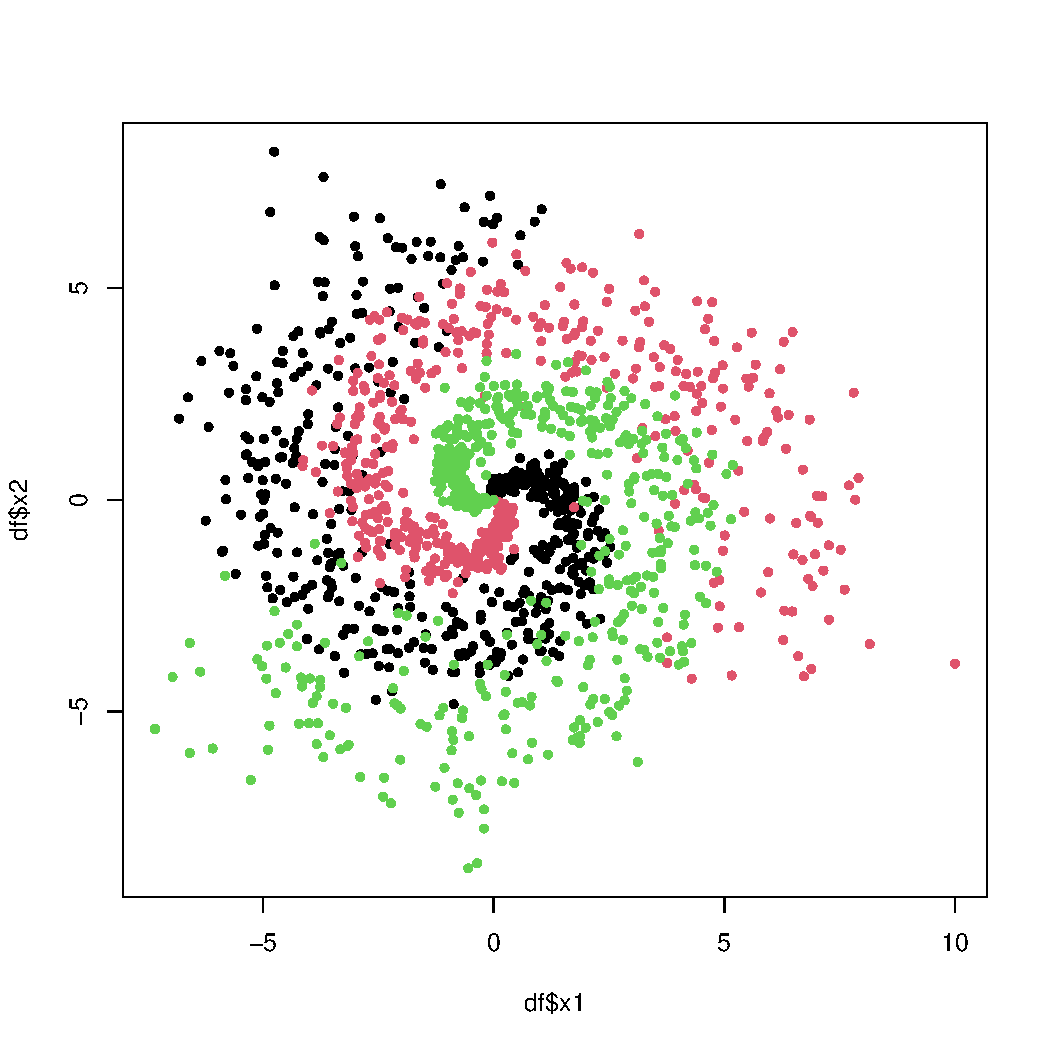
\includegraphics{hw5_files/figure-pdf/unnamed-chunk-26-1.pdf}

}

\end{figure}

Define a grid of \(100\) points from \(-10\) to \(10\) in both \(x_1\)
and \(x_2\) using the \texttt{expand.grid()}. Save it as a tibble called
\texttt{df\_test}.

\begin{Shaded}
\begin{Highlighting}[]
\NormalTok{generate\_three\_spirals }\OtherTok{\textless{}{-}} \ControlFlowTok{function}\NormalTok{() \{}
  \FunctionTok{set.seed}\NormalTok{(}\DecValTok{42}\NormalTok{)}
\NormalTok{  n }\OtherTok{\textless{}{-}} \DecValTok{500}
\NormalTok{  noise }\OtherTok{\textless{}{-}} \FloatTok{0.2}
\NormalTok{  t }\OtherTok{\textless{}{-}}\NormalTok{ (}\DecValTok{1}\SpecialCharTok{:}\NormalTok{n) }\SpecialCharTok{/}\NormalTok{ n }\SpecialCharTok{*} \DecValTok{2} \SpecialCharTok{*}\NormalTok{ pi}
\NormalTok{  x1 }\OtherTok{\textless{}{-}} \FunctionTok{c}\NormalTok{(}
\NormalTok{    t }\SpecialCharTok{*}\NormalTok{ (}\FunctionTok{sin}\NormalTok{(t) }\SpecialCharTok{+} \FunctionTok{rnorm}\NormalTok{(n, }\DecValTok{0}\NormalTok{, noise)),}
\NormalTok{    t }\SpecialCharTok{*}\NormalTok{ (}\FunctionTok{sin}\NormalTok{(t }\SpecialCharTok{+} \DecValTok{2} \SpecialCharTok{*}\NormalTok{ pi}\SpecialCharTok{/}\DecValTok{3}\NormalTok{) }\SpecialCharTok{+} \FunctionTok{rnorm}\NormalTok{(n, }\DecValTok{0}\NormalTok{, noise)),}
\NormalTok{    t }\SpecialCharTok{*}\NormalTok{ (}\FunctionTok{sin}\NormalTok{(t }\SpecialCharTok{+} \DecValTok{4} \SpecialCharTok{*}\NormalTok{ pi}\SpecialCharTok{/}\DecValTok{3}\NormalTok{) }\SpecialCharTok{+} \FunctionTok{rnorm}\NormalTok{(n, }\DecValTok{0}\NormalTok{, noise))}
\NormalTok{  )}
\NormalTok{  x2 }\OtherTok{\textless{}{-}} \FunctionTok{c}\NormalTok{(}
\NormalTok{    t }\SpecialCharTok{*}\NormalTok{ (}\FunctionTok{cos}\NormalTok{(t) }\SpecialCharTok{+} \FunctionTok{rnorm}\NormalTok{(n, }\DecValTok{0}\NormalTok{, noise)),}
\NormalTok{    t }\SpecialCharTok{*}\NormalTok{ (}\FunctionTok{cos}\NormalTok{(t }\SpecialCharTok{+} \DecValTok{2} \SpecialCharTok{*}\NormalTok{ pi}\SpecialCharTok{/}\DecValTok{3}\NormalTok{) }\SpecialCharTok{+} \FunctionTok{rnorm}\NormalTok{(n, }\DecValTok{0}\NormalTok{, noise)),}
\NormalTok{    t }\SpecialCharTok{*}\NormalTok{ (}\FunctionTok{cos}\NormalTok{(t }\SpecialCharTok{+} \DecValTok{4} \SpecialCharTok{*}\NormalTok{ pi}\SpecialCharTok{/}\DecValTok{3}\NormalTok{) }\SpecialCharTok{+} \FunctionTok{rnorm}\NormalTok{(n, }\DecValTok{0}\NormalTok{, noise))}
\NormalTok{  )}
\NormalTok{  y }\OtherTok{\textless{}{-}} \FunctionTok{factor}\NormalTok{(}
    \FunctionTok{c}\NormalTok{(}\FunctionTok{rep}\NormalTok{(}\DecValTok{0}\NormalTok{, n), }\FunctionTok{rep}\NormalTok{(}\DecValTok{1}\NormalTok{, n), }\FunctionTok{rep}\NormalTok{(}\DecValTok{2}\NormalTok{, n))}
\NormalTok{  )}
  \FunctionTok{return}\NormalTok{(tibble}\SpecialCharTok{::}\FunctionTok{tibble}\NormalTok{(}\AttributeTok{x1=}\NormalTok{x1, }\AttributeTok{x2=}\NormalTok{x2, }\AttributeTok{y=}\NormalTok{y))}
\NormalTok{\}}

\NormalTok{df }\OtherTok{\textless{}{-}} \FunctionTok{generate\_three\_spirals}\NormalTok{()}
\FunctionTok{plot}\NormalTok{(df}\SpecialCharTok{$}\NormalTok{x1, df}\SpecialCharTok{$}\NormalTok{x2, }\AttributeTok{col=}\NormalTok{df}\SpecialCharTok{$}\NormalTok{y, }\AttributeTok{pch=}\DecValTok{20}\NormalTok{)}
\end{Highlighting}
\end{Shaded}

\begin{figure}[H]

{\centering 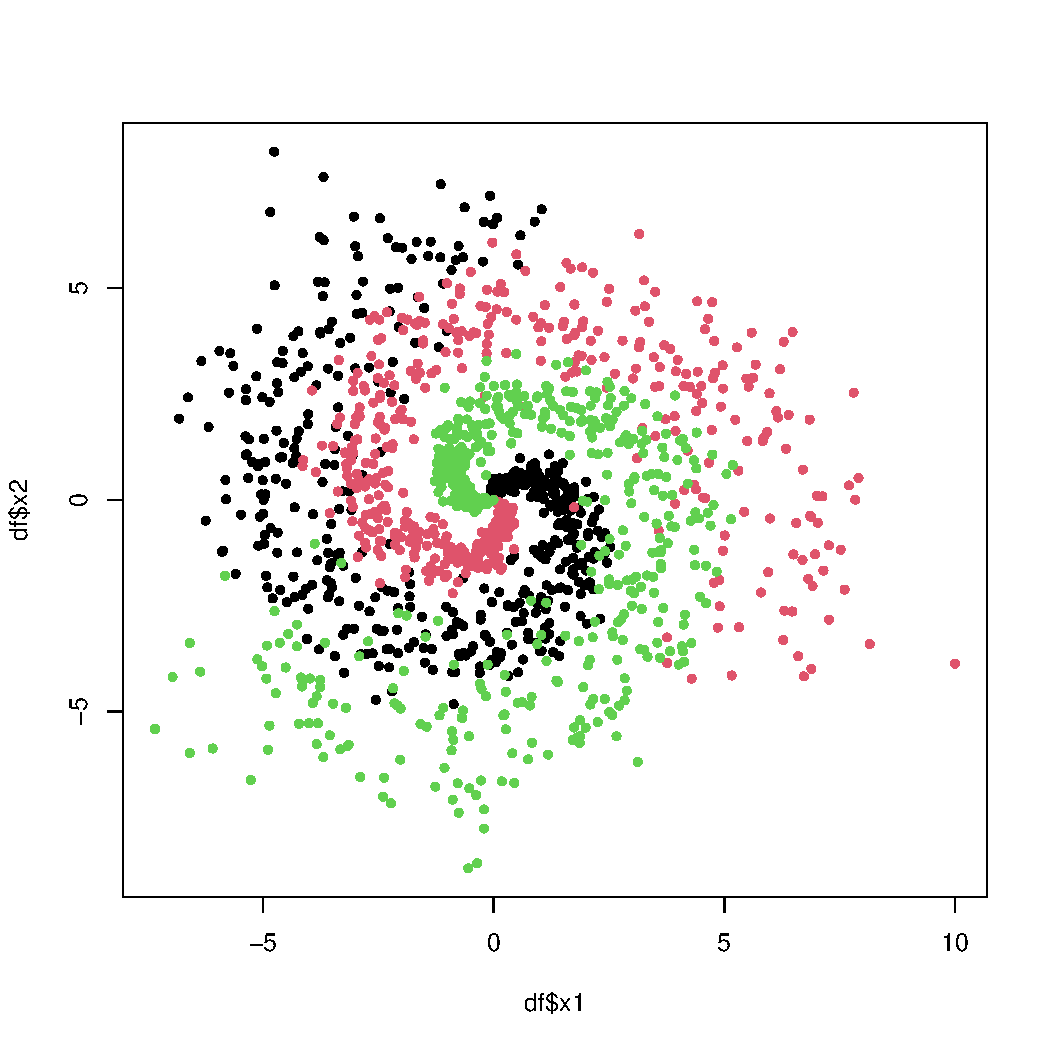
\includegraphics{hw5_files/figure-pdf/unnamed-chunk-27-1.pdf}

}

\end{figure}

\begin{Shaded}
\begin{Highlighting}[]
\NormalTok{grid }\OtherTok{\textless{}{-}} \FunctionTok{expand.grid}\NormalTok{(}\AttributeTok{x1 =} \FunctionTok{seq}\NormalTok{(}\SpecialCharTok{{-}}\DecValTok{10}\NormalTok{, }\DecValTok{10}\NormalTok{, }\AttributeTok{length.out =} \DecValTok{100}\NormalTok{), }
                    \AttributeTok{x2 =} \FunctionTok{seq}\NormalTok{(}\SpecialCharTok{{-}}\DecValTok{10}\NormalTok{, }\DecValTok{10}\NormalTok{, }\AttributeTok{length.out =} \DecValTok{100}\NormalTok{))}

\NormalTok{df\_test }\OtherTok{\textless{}{-}}\NormalTok{ tibble}\SpecialCharTok{::}\FunctionTok{as\_tibble}\NormalTok{(grid)}
\end{Highlighting}
\end{Shaded}

\begin{center}\rule{0.5\linewidth}{0.5pt}\end{center}

3.2 (10 points)

Fit a classification tree model to predict the \texttt{y} variable using
the \texttt{x1} and \texttt{x2} predictors, and plot the decision
boundary.

Plot the decision boundary using the following function:

\begin{Shaded}
\begin{Highlighting}[]
\FunctionTok{library}\NormalTok{(rpart)}

\NormalTok{rpart\_fit }\OtherTok{\textless{}{-}} \FunctionTok{rpart}\NormalTok{(y }\SpecialCharTok{\textasciitilde{}}\NormalTok{ x1 }\SpecialCharTok{+}\NormalTok{ x2, }\AttributeTok{data=}\NormalTok{df, }\AttributeTok{method=}\StringTok{"class"}\NormalTok{)}

\NormalTok{df\_test}\SpecialCharTok{$}\NormalTok{predictions }\OtherTok{\textless{}{-}} \FunctionTok{predict}\NormalTok{(rpart\_fit, }\AttributeTok{newdata=}\NormalTok{df\_test, }\AttributeTok{type=}\StringTok{"class"}\NormalTok{)}

\NormalTok{plot\_decision\_boundary }\OtherTok{\textless{}{-}} \ControlFlowTok{function}\NormalTok{(predictions)\{}
  \FunctionTok{plot}\NormalTok{(}
\NormalTok{    df\_test}\SpecialCharTok{$}\NormalTok{x1, df\_test}\SpecialCharTok{$}\NormalTok{x2,}
    \AttributeTok{col =} \FunctionTok{as.numeric}\NormalTok{(predictions),}
    \AttributeTok{pch =} \DecValTok{16}\NormalTok{,}
    \AttributeTok{cex =} \FloatTok{0.6}\NormalTok{,}
    \AttributeTok{xlab =} \StringTok{"x1"}\NormalTok{,}
    \AttributeTok{ylab =} \StringTok{"x2"}\NormalTok{,}
    \AttributeTok{main =} \StringTok{"Decision Boundary"}
\NormalTok{  )}
  \FunctionTok{points}\NormalTok{(}
\NormalTok{    df}\SpecialCharTok{$}\NormalTok{x1, df}\SpecialCharTok{$}\NormalTok{x2,}
    \AttributeTok{col =} \FunctionTok{as.numeric}\NormalTok{(df}\SpecialCharTok{$}\NormalTok{y),}
    \AttributeTok{pch =} \DecValTok{20}
\NormalTok{  )}
\NormalTok{\}}

\FunctionTok{plot\_decision\_boundary}\NormalTok{(df\_test}\SpecialCharTok{$}\NormalTok{predictions)}
\end{Highlighting}
\end{Shaded}

\begin{figure}[H]

{\centering 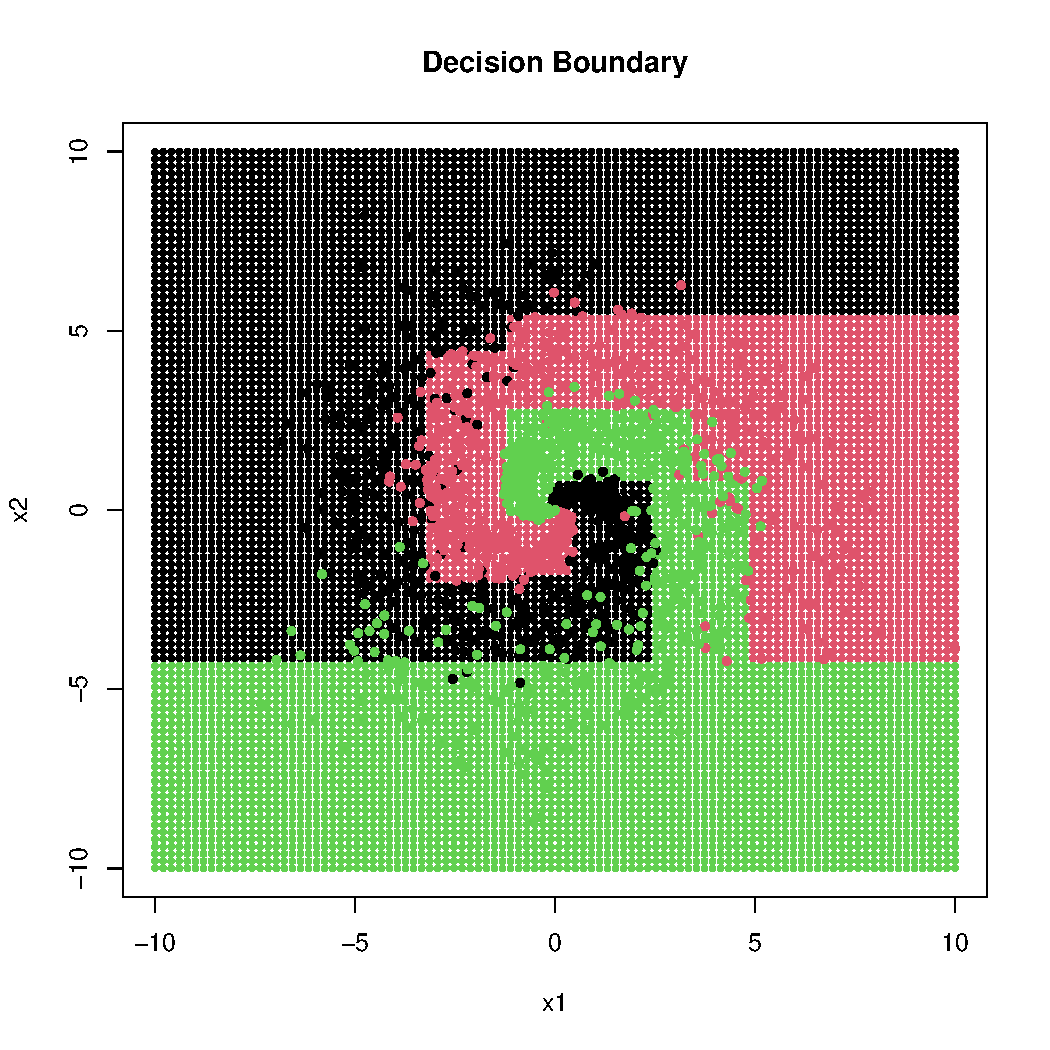
\includegraphics{hw5_files/figure-pdf/unnamed-chunk-28-1.pdf}

}

\end{figure}

\begin{center}\rule{0.5\linewidth}{0.5pt}\end{center}

3.3 (10 points)

Fit a support vector machine model to predict the \texttt{y} variable
using the \texttt{x1} and \texttt{x2} predictors. Use the \texttt{svm()}
function and use any kernel of your choice. Remember to set the
\texttt{type} argument to \texttt{"C-classification"} \textbf{if you
haven't} converted \texttt{y} to be of type \texttt{factor}.

\begin{Shaded}
\begin{Highlighting}[]
\NormalTok{svm\_fit }\OtherTok{\textless{}{-}}\NormalTok{ ... }\CommentTok{\# Insert your code here}
\NormalTok{svm\_classes }\OtherTok{\textless{}{-}}\NormalTok{ ... }\CommentTok{\# Insert your code here}
\FunctionTok{plot\_decision\_boundary}\NormalTok{(svm\_classes)}
\end{Highlighting}
\end{Shaded}

\begin{Shaded}
\begin{Highlighting}[]
\FunctionTok{library}\NormalTok{(e1071)}

\NormalTok{svm\_fit }\OtherTok{\textless{}{-}} \FunctionTok{svm}\NormalTok{(y }\SpecialCharTok{\textasciitilde{}}\NormalTok{ x1 }\SpecialCharTok{+}\NormalTok{ x2, }\AttributeTok{data =}\NormalTok{ df, }\AttributeTok{type =} \StringTok{"C{-}classification"}\NormalTok{, }\AttributeTok{kernel =} \StringTok{"radial"}\NormalTok{)}

\NormalTok{svm\_classes }\OtherTok{\textless{}{-}} \FunctionTok{predict}\NormalTok{(svm\_fit, }\AttributeTok{newdata =}\NormalTok{ df\_test)}

\FunctionTok{plot\_decision\_boundary}\NormalTok{(svm\_classes)}
\end{Highlighting}
\end{Shaded}

\begin{figure}[H]

{\centering 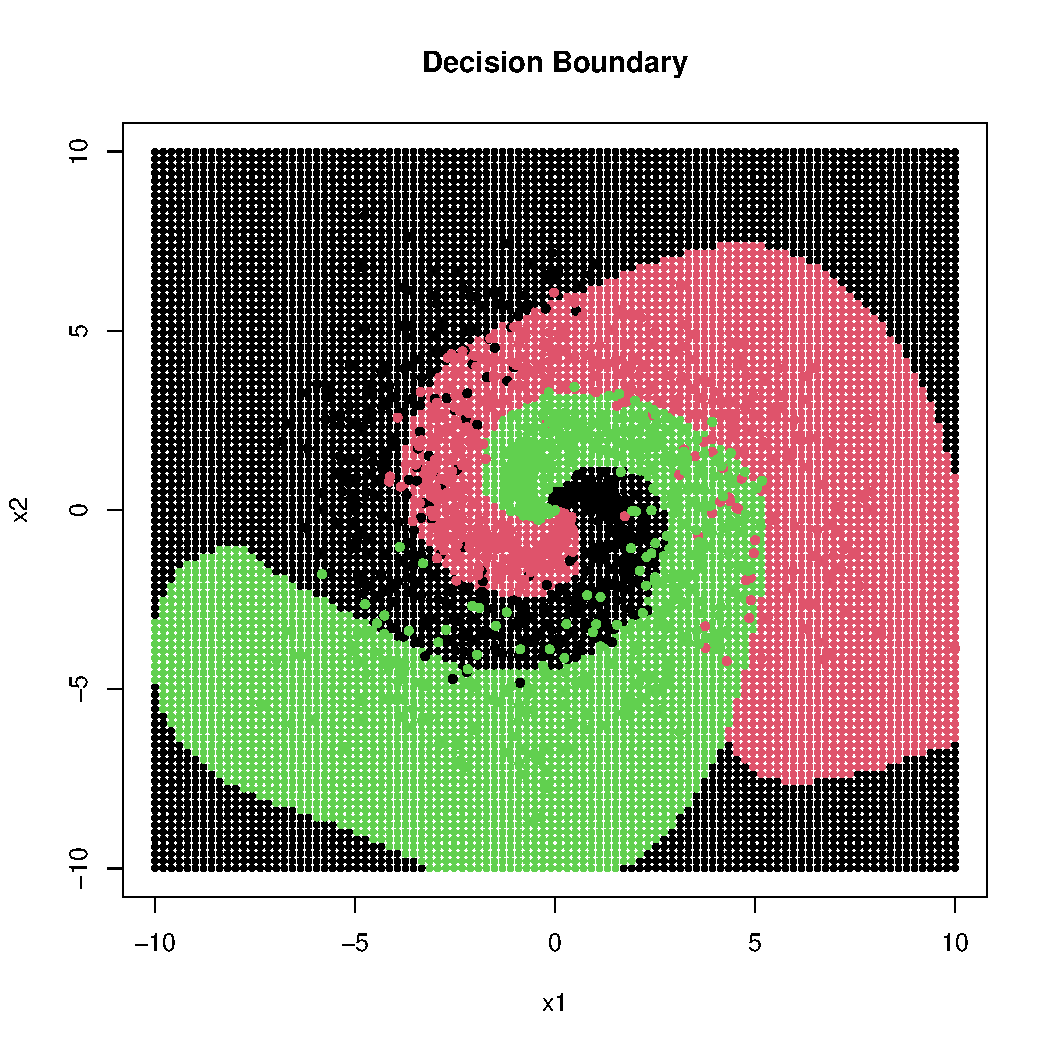
\includegraphics{hw5_files/figure-pdf/unnamed-chunk-29-1.pdf}

}

\end{figure}

\begin{center}\rule{0.5\linewidth}{0.5pt}\end{center}

\begin{tcolorbox}[enhanced jigsaw, bottomtitle=1mm, rightrule=.15mm, left=2mm, colback=white, opacityback=0, bottomrule=.15mm, titlerule=0mm, toprule=.15mm, colframe=quarto-callout-warning-color-frame, arc=.35mm, colbacktitle=quarto-callout-warning-color!10!white, breakable, leftrule=.75mm, coltitle=black, title=\textcolor{quarto-callout-warning-color}{\faExclamationTriangle}\hspace{0.5em}{Instructions}, opacitybacktitle=0.6, toptitle=1mm]

For the next questions, you will need to fit a series of neural
networks. In all cases, you can:

\begin{itemize}
\tightlist
\item
  set the number of units in each hidden layer to 10
\item
  set the output dimension \texttt{o} to 3 (remember this is multinomial
  classification)
\item
  use the appropriate loss function for the problem (\textbf{not
  \texttt{nn\_bce\_loss}})
\item
  set the number of epochs to \(50\)
\item
  fit the model using the \texttt{luz} package
\end{itemize}

You can use any optimizer of your choice, but you \textbf{will need to
tune the learning rate for each problem}.

\end{tcolorbox}

3.4 (10 points)

Fit a neural network with \textbf{1 hidden layer} to predict the
\texttt{y} variable using the \texttt{x1} and \texttt{x2} predictors.

In order to generate the class predictions, you will need to use the

Plot the results using the \texttt{plot\_decision\_boundary()} function.

\begin{Shaded}
\begin{Highlighting}[]
\FunctionTok{library}\NormalTok{(torch)}
\FunctionTok{library}\NormalTok{(luz)}

\CommentTok{\# Define the neural network with one hidden layer}
\NormalTok{NN1 }\OtherTok{\textless{}{-}} \FunctionTok{nn\_module}\NormalTok{(}
  \AttributeTok{initialize =} \ControlFlowTok{function}\NormalTok{(p, q1, o) \{}
\NormalTok{    self}\SpecialCharTok{$}\NormalTok{hidden1 }\OtherTok{\textless{}{-}} \FunctionTok{nn\_linear}\NormalTok{(p, q1) }\CommentTok{\# first hidden layer}
\NormalTok{    self}\SpecialCharTok{$}\NormalTok{output }\OtherTok{\textless{}{-}} \FunctionTok{nn\_linear}\NormalTok{(q1, o) }\CommentTok{\# output layer}
\NormalTok{    self}\SpecialCharTok{$}\NormalTok{activation }\OtherTok{\textless{}{-}} \FunctionTok{nn\_relu}\NormalTok{() }\CommentTok{\# ReLU activation function}
\NormalTok{  \},}
  \AttributeTok{forward =} \ControlFlowTok{function}\NormalTok{(x) \{}
\NormalTok{    x }\SpecialCharTok{\%\textgreater{}\%}
\NormalTok{      self}\SpecialCharTok{$}\FunctionTok{hidden1}\NormalTok{() }\SpecialCharTok{\%\textgreater{}\%}
\NormalTok{      self}\SpecialCharTok{$}\FunctionTok{activation}\NormalTok{() }\SpecialCharTok{\%\textgreater{}\%}
\NormalTok{      self}\SpecialCharTok{$}\FunctionTok{output}\NormalTok{()}
\NormalTok{  \}}
\NormalTok{)}

\CommentTok{\# Instantiate the model}
\CommentTok{\# Assuming \textasciigrave{}p\textasciigrave{} is the number of input features, \textasciigrave{}q1\textasciigrave{} is the number of units in the hidden layer, and \textasciigrave{}o\textasciigrave{} is the number of output units/classes}
\NormalTok{p }\OtherTok{\textless{}{-}} \DecValTok{2} \CommentTok{\# because we have 2 predictors: x1 and x2}
\NormalTok{q1 }\OtherTok{\textless{}{-}} \DecValTok{10} \CommentTok{\# number of units in the hidden layer}
\NormalTok{o }\OtherTok{\textless{}{-}} \DecValTok{3} \CommentTok{\# number of classes for output}
\end{Highlighting}
\end{Shaded}

\begin{Shaded}
\begin{Highlighting}[]
\CommentTok{\# Train the model}
\NormalTok{fit\_1 }\OtherTok{\textless{}{-}}\NormalTok{ NN1 }\SpecialCharTok{\%\textgreater{}\%}
  \FunctionTok{setup}\NormalTok{(}
    \AttributeTok{loss =} \FunctionTok{nn\_cross\_entropy\_loss}\NormalTok{(), }\CommentTok{\# Cross{-}entropy loss for classification}
    \AttributeTok{optimizer =}\NormalTok{ optim\_adam, }\CommentTok{\# Adam optimizer}
    
\NormalTok{  ) }\SpecialCharTok{\%\textgreater{}\%}
  \FunctionTok{set\_hparams}\NormalTok{(}
    \AttributeTok{p =}\NormalTok{ p,}
    \AttributeTok{q1 =}\NormalTok{ q1,}
    \AttributeTok{o =}\NormalTok{ o}
\NormalTok{  ) }\SpecialCharTok{\%\textgreater{}\%}
  \FunctionTok{set\_opt\_hparams}\NormalTok{(}\AttributeTok{lr =} \FloatTok{0.01}\NormalTok{) }\SpecialCharTok{\%\textgreater{}\%}   \CommentTok{\# Learning rate}
  \FunctionTok{fit}\NormalTok{(}
    \AttributeTok{data =} \FunctionTok{list}\NormalTok{(}
      \AttributeTok{x =}\NormalTok{ df }\SpecialCharTok{\%\textgreater{}\%} \FunctionTok{select}\NormalTok{(x1, x2) }\SpecialCharTok{\%\textgreater{}\%} \FunctionTok{as.matrix}\NormalTok{(),}
      \AttributeTok{y =}\NormalTok{ df}\SpecialCharTok{$}\NormalTok{y }\SpecialCharTok{\%\textgreater{}\%} \FunctionTok{as.integer}\NormalTok{()}
\NormalTok{    ),}
    \AttributeTok{epochs =} \DecValTok{50}\NormalTok{,}
    \AttributeTok{dataloader\_options =} \FunctionTok{list}\NormalTok{(}\AttributeTok{batch\_size =} \DecValTok{64}\NormalTok{), }\CommentTok{\# options for the data loader}
    \AttributeTok{valid\_data =} \FloatTok{0.2}\NormalTok{, }
    \AttributeTok{verbose =} \ConstantTok{FALSE}
\NormalTok{  )}
\end{Highlighting}
\end{Shaded}

\begin{Shaded}
\begin{Highlighting}[]
\FunctionTok{plot}\NormalTok{(fit\_1)}
\end{Highlighting}
\end{Shaded}

\begin{figure}[H]

{\centering 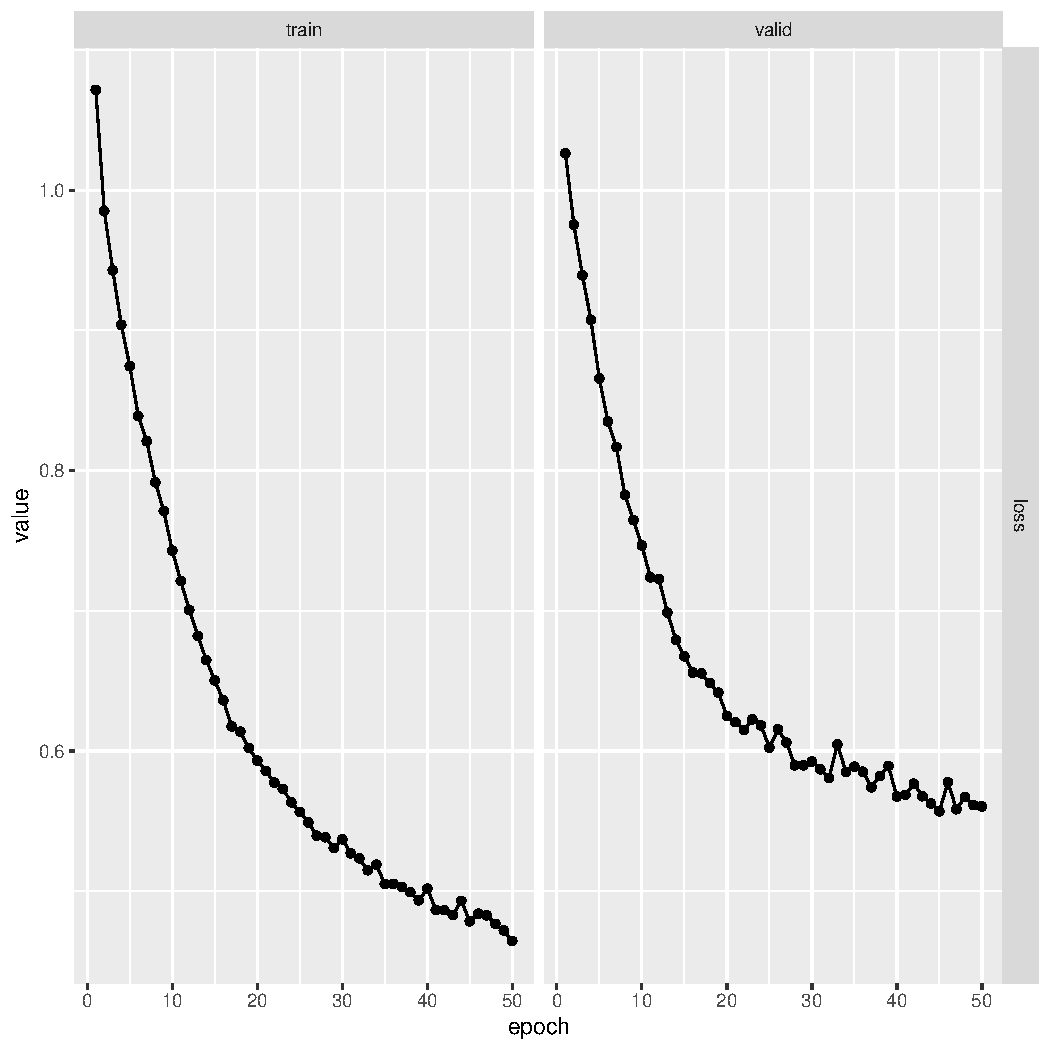
\includegraphics{hw5_files/figure-pdf/unnamed-chunk-32-1.pdf}

}

\end{figure}

\begin{Shaded}
\begin{Highlighting}[]
\CommentTok{\# Predict using the model}
\NormalTok{test\_matrix }\OtherTok{\textless{}{-}}\NormalTok{ df\_test }\SpecialCharTok{\%\textgreater{}\%} \FunctionTok{select}\NormalTok{(x1, x2) }\SpecialCharTok{\%\textgreater{}\%} \FunctionTok{as.matrix}\NormalTok{()}
\NormalTok{fit\_1\_predictions }\OtherTok{\textless{}{-}} \FunctionTok{predict}\NormalTok{(fit\_1, test\_matrix) }\SpecialCharTok{\%\textgreater{}\%}
  \FunctionTok{torch\_argmax}\NormalTok{(}\AttributeTok{dim =} \DecValTok{2}\NormalTok{) }\SpecialCharTok{\%\textgreater{}\%}
  \FunctionTok{as.integer}\NormalTok{()}

\CommentTok{\# Plot the decision boundary}
\FunctionTok{plot\_decision\_boundary}\NormalTok{(fit\_1\_predictions)}
\end{Highlighting}
\end{Shaded}

\begin{figure}[H]

{\centering 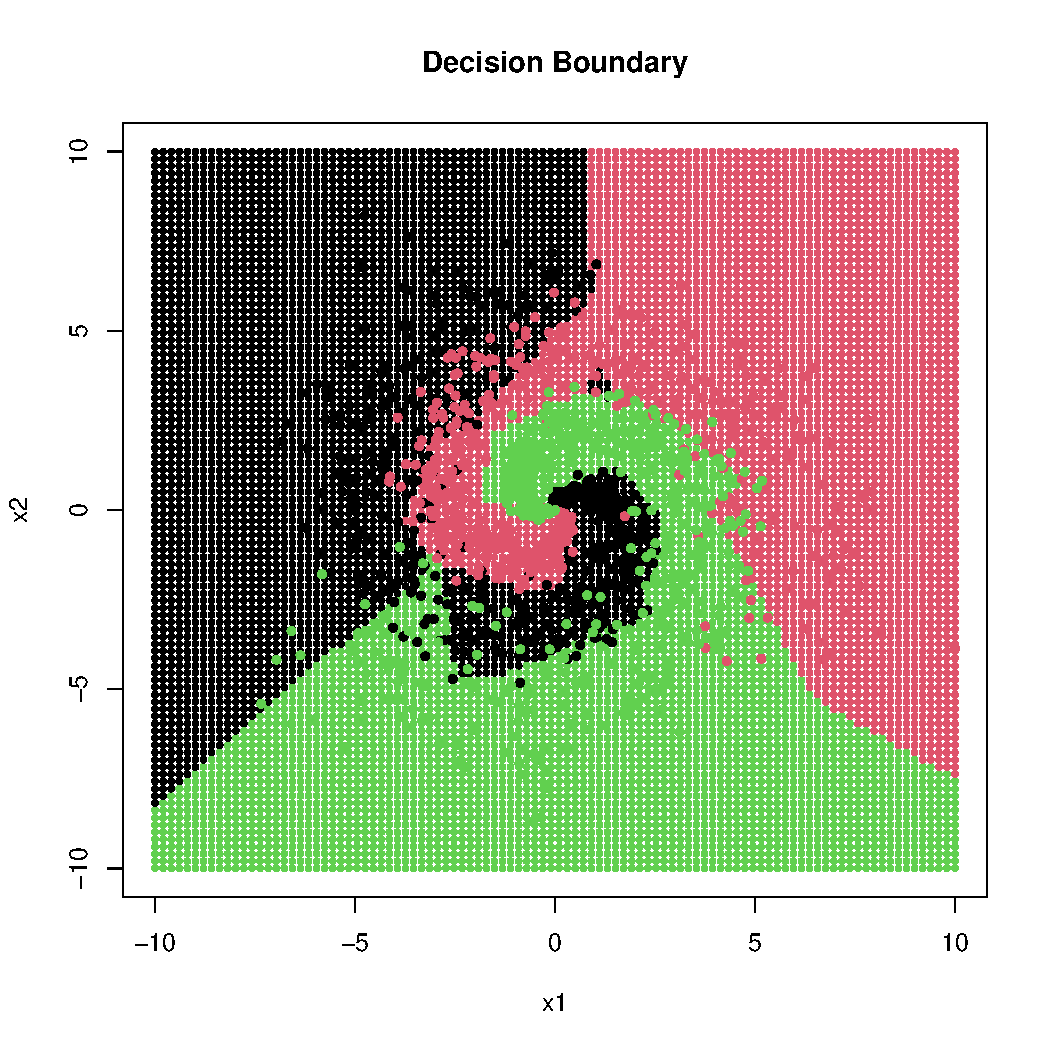
\includegraphics{hw5_files/figure-pdf/unnamed-chunk-32-2.pdf}

}

\end{figure}

\begin{center}\rule{0.5\linewidth}{0.5pt}\end{center}

3.5 (10 points)

Fit a neural network with \textbf{0 hidden layers} to predict the
\texttt{y} variable using the \texttt{x1} and \texttt{x2} predictors.

\begin{Shaded}
\begin{Highlighting}[]
\NormalTok{NN0 }\OtherTok{\textless{}{-}} \FunctionTok{nn\_module}\NormalTok{(}
  \AttributeTok{initialize =} \ControlFlowTok{function}\NormalTok{(p, o)\{}
\NormalTok{    ... }\CommentTok{\# Insert your code here}
\NormalTok{  \},}
  \AttributeTok{forward =} \ControlFlowTok{function}\NormalTok{(x)\{}
\NormalTok{    x }\SpecialCharTok{\%\textgreater{}\%} 
\NormalTok{    ... }\CommentTok{\# Insert your code here}
\NormalTok{  \}}
\NormalTok{)}

\NormalTok{fit\_0 }\OtherTok{\textless{}{-}}\NormalTok{ NN0 }\SpecialCharTok{\%\textgreater{}\%} 
  \FunctionTok{setup}\NormalTok{(...) }\SpecialCharTok{\%\textgreater{}\%}
  \FunctionTok{set\_hparams}\NormalTok{(...) }\SpecialCharTok{\%\textgreater{}\%}
  \FunctionTok{set\_opt\_params}\NormalTok{(...) }\SpecialCharTok{\%\textgreater{}\%}
  \FunctionTok{fit}\NormalTok{(...)}
\end{Highlighting}
\end{Shaded}

Plot the results using the \texttt{plot\_decision\_boundary()} function.

\begin{Shaded}
\begin{Highlighting}[]
\FunctionTok{library}\NormalTok{(torch)}
\FunctionTok{library}\NormalTok{(luz)}

\CommentTok{\# 定义无隐藏层的NN模型}
\NormalTok{NN0 }\OtherTok{\textless{}{-}} \FunctionTok{nn\_module}\NormalTok{(}
  \AttributeTok{initialize =} \ControlFlowTok{function}\NormalTok{(p, o) \{}
\NormalTok{    self}\SpecialCharTok{$}\NormalTok{output }\OtherTok{\textless{}{-}} \FunctionTok{nn\_linear}\NormalTok{(p, o) }\CommentTok{\# p是输入特征的数量,o是输出类别的数量}
\NormalTok{  \},}
  \AttributeTok{forward =} \ControlFlowTok{function}\NormalTok{(x) \{}
\NormalTok{    x }\SpecialCharTok{\%\textgreater{}\%} 
\NormalTok{      self}\SpecialCharTok{$}\FunctionTok{output}\NormalTok{()}
\NormalTok{  \}}
\NormalTok{)}

\CommentTok{\# 设置模型参数}
\NormalTok{p }\OtherTok{\textless{}{-}} \DecValTok{2} \CommentTok{\# 因为有x1和x2两个输入}
\NormalTok{o }\OtherTok{\textless{}{-}} \DecValTok{3} \CommentTok{\# 假设有3个不同的类别}


\CommentTok{\# 训练无隐藏层的NN模型}
\NormalTok{fit\_0 }\OtherTok{\textless{}{-}}\NormalTok{ NN0 }\SpecialCharTok{\%\textgreater{}\%}
  \FunctionTok{setup}\NormalTok{(}
    \AttributeTok{loss =} \FunctionTok{nn\_cross\_entropy\_loss}\NormalTok{(), }\CommentTok{\# 使用交叉熵损失函数}
    \AttributeTok{optimizer =}\NormalTok{ optim\_adam, }\CommentTok{\# 传递优化器的函数引用}
    
\NormalTok{  ) }\SpecialCharTok{\%\textgreater{}\%}
  \FunctionTok{set\_hparams}\NormalTok{(}
    \AttributeTok{p =}\NormalTok{ p,}
    \AttributeTok{o =}\NormalTok{ o}
\NormalTok{  ) }\SpecialCharTok{\%\textgreater{}\%}
  \FunctionTok{set\_opt\_hparams}\NormalTok{(}\AttributeTok{lr =} \FloatTok{0.01}\NormalTok{) }\SpecialCharTok{\%\textgreater{}\%}
  \FunctionTok{fit}\NormalTok{(}
    \AttributeTok{data =} \FunctionTok{list}\NormalTok{(}
      \AttributeTok{x =}\NormalTok{ df }\SpecialCharTok{\%\textgreater{}\%} \FunctionTok{select}\NormalTok{(x1, x2) }\SpecialCharTok{\%\textgreater{}\%} \FunctionTok{as.matrix}\NormalTok{(), }\CommentTok{\# 训练数据}
      \AttributeTok{y =}\NormalTok{ df}\SpecialCharTok{$}\NormalTok{y }\SpecialCharTok{\%\textgreater{}\%} \FunctionTok{as.integer}\NormalTok{() }\CommentTok{\# 类别标签}
\NormalTok{    ),}
    \AttributeTok{epochs =} \DecValTok{50}\NormalTok{, }\CommentTok{\# 设置训练周期为50}
    \AttributeTok{valid\_data =} \FloatTok{0.2}\NormalTok{,}
    \AttributeTok{dataloader\_options =} \FunctionTok{list}\NormalTok{(}\AttributeTok{batch\_size =} \DecValTok{64}\NormalTok{), }\CommentTok{\# 确保批处理大小为64}
    \AttributeTok{verbose =} \ConstantTok{FALSE}
\NormalTok{  )}
\end{Highlighting}
\end{Shaded}

\begin{Shaded}
\begin{Highlighting}[]
\FunctionTok{plot}\NormalTok{(fit\_0)}
\end{Highlighting}
\end{Shaded}

\begin{figure}[H]

{\centering 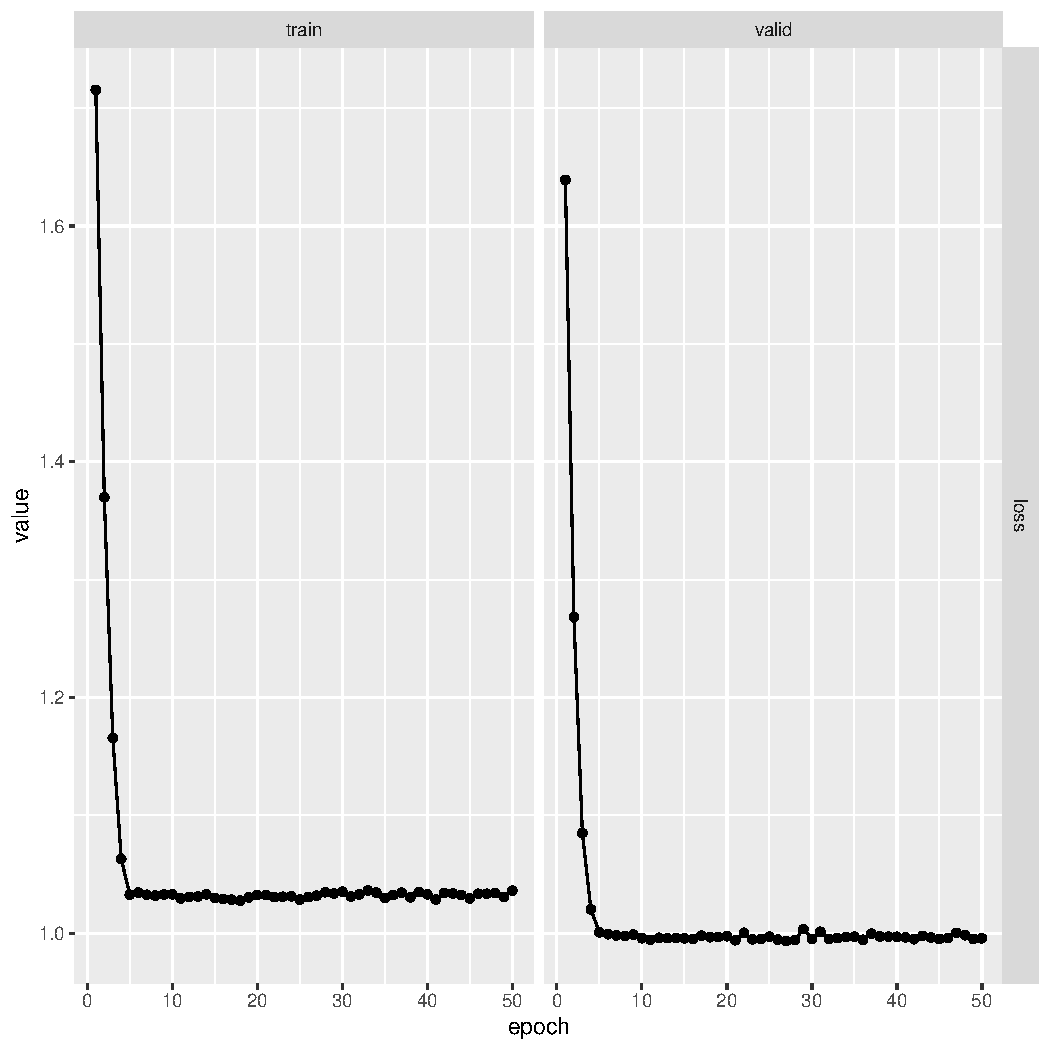
\includegraphics{hw5_files/figure-pdf/unnamed-chunk-34-1.pdf}

}

\end{figure}

\begin{Shaded}
\begin{Highlighting}[]
\CommentTok{\# 生成预测并绘制决策边界}
\NormalTok{test\_matrix }\OtherTok{\textless{}{-}}\NormalTok{ df\_test }\SpecialCharTok{\%\textgreater{}\%} \FunctionTok{select}\NormalTok{(x1, x2) }\SpecialCharTok{\%\textgreater{}\%} \FunctionTok{as.matrix}\NormalTok{()}
\NormalTok{fit\_0\_predictions }\OtherTok{\textless{}{-}} \FunctionTok{predict}\NormalTok{(fit\_0, test\_matrix) }\SpecialCharTok{\%\textgreater{}\%}
  \FunctionTok{torch\_argmax}\NormalTok{(}\AttributeTok{dim =} \DecValTok{2}\NormalTok{) }\SpecialCharTok{\%\textgreater{}\%}
  \FunctionTok{as.integer}\NormalTok{()}


\FunctionTok{plot\_decision\_boundary}\NormalTok{(fit\_0\_predictions)}
\end{Highlighting}
\end{Shaded}

\begin{figure}[H]

{\centering 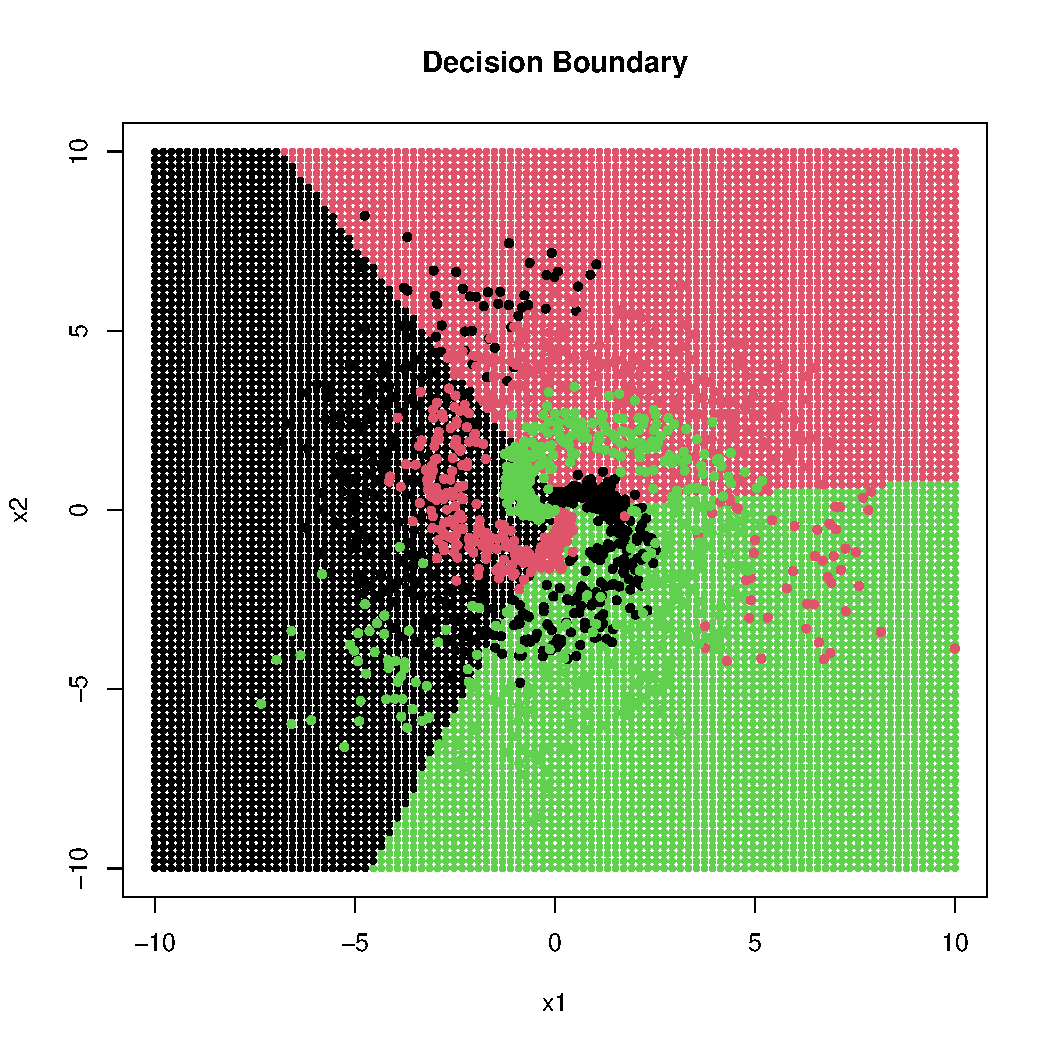
\includegraphics{hw5_files/figure-pdf/unnamed-chunk-34-2.pdf}

}

\end{figure}

\begin{center}\rule{0.5\linewidth}{0.5pt}\end{center}

3.6 (10 points)

Fit a neural network with \textbf{3 hidden layers} to predict the
\texttt{y} variable using the \texttt{x1} and \texttt{x2} predictors.

\begin{Shaded}
\begin{Highlighting}[]
\NormalTok{NN2 }\OtherTok{\textless{}{-}} \FunctionTok{nn\_module}\NormalTok{(}
  \AttributeTok{initialize =} \ControlFlowTok{function}\NormalTok{(p, q1, q2, o)\{}
\NormalTok{    ... }\CommentTok{\# Insert your code here}
\NormalTok{  \},}
  \AttributeTok{forward =} \ControlFlowTok{function}\NormalTok{(x)\{}
\NormalTok{    x }\SpecialCharTok{\%\textgreater{}\%} 
\NormalTok{    ... }\CommentTok{\# Insert your code here}
\NormalTok{  \}}
\NormalTok{)}

\NormalTok{fit\_2 }\OtherTok{\textless{}{-}}\NormalTok{ NN3 }\SpecialCharTok{\%\textgreater{}\%} 
  \FunctionTok{setup}\NormalTok{(...) }\SpecialCharTok{\%\textgreater{}\%}
  \FunctionTok{set\_hparams}\NormalTok{(...) }\SpecialCharTok{\%\textgreater{}\%}
  \FunctionTok{set\_opt\_params}\NormalTok{(...) }\SpecialCharTok{\%\textgreater{}\%}
  \FunctionTok{fit}\NormalTok{(...)}
\end{Highlighting}
\end{Shaded}

Plot the results using the \texttt{plot\_decision\_boundary()} function.

\begin{Shaded}
\begin{Highlighting}[]
\FunctionTok{library}\NormalTok{(torch)}
\FunctionTok{library}\NormalTok{(luz)}

\CommentTok{\# 定义带有三个隐藏层的NN模型}
\NormalTok{NN3 }\OtherTok{\textless{}{-}} \FunctionTok{nn\_module}\NormalTok{(}
  \AttributeTok{initialize =} \ControlFlowTok{function}\NormalTok{(p, q1, q2, q3, o) \{}
\NormalTok{    self}\SpecialCharTok{$}\NormalTok{hidden1 }\OtherTok{\textless{}{-}} \FunctionTok{nn\_linear}\NormalTok{(p, q1)}
\NormalTok{    self}\SpecialCharTok{$}\NormalTok{hidden2 }\OtherTok{\textless{}{-}} \FunctionTok{nn\_linear}\NormalTok{(q1, q2)}
\NormalTok{    self}\SpecialCharTok{$}\NormalTok{hidden3 }\OtherTok{\textless{}{-}} \FunctionTok{nn\_linear}\NormalTok{(q2, q3)}
\NormalTok{    self}\SpecialCharTok{$}\NormalTok{output }\OtherTok{\textless{}{-}} \FunctionTok{nn\_linear}\NormalTok{(q3, o)}
\NormalTok{    self}\SpecialCharTok{$}\NormalTok{activation }\OtherTok{\textless{}{-}} \FunctionTok{nn\_relu}\NormalTok{()}
\NormalTok{  \},}
  \AttributeTok{forward =} \ControlFlowTok{function}\NormalTok{(x) \{}
\NormalTok{    x }\SpecialCharTok{\%\textgreater{}\%}
\NormalTok{      self}\SpecialCharTok{$}\FunctionTok{hidden1}\NormalTok{() }\SpecialCharTok{\%\textgreater{}\%}
\NormalTok{      self}\SpecialCharTok{$}\FunctionTok{activation}\NormalTok{() }\SpecialCharTok{\%\textgreater{}\%}
\NormalTok{      self}\SpecialCharTok{$}\FunctionTok{hidden2}\NormalTok{() }\SpecialCharTok{\%\textgreater{}\%}
\NormalTok{      self}\SpecialCharTok{$}\FunctionTok{activation}\NormalTok{() }\SpecialCharTok{\%\textgreater{}\%}
\NormalTok{      self}\SpecialCharTok{$}\FunctionTok{hidden3}\NormalTok{() }\SpecialCharTok{\%\textgreater{}\%}
\NormalTok{      self}\SpecialCharTok{$}\FunctionTok{activation}\NormalTok{() }\SpecialCharTok{\%\textgreater{}\%}
\NormalTok{      self}\SpecialCharTok{$}\FunctionTok{output}\NormalTok{()}
\NormalTok{  \}}
\NormalTok{)}

\CommentTok{\# 实例化NN3模型}
\CommentTok{\# 假设我们有以下参数:p是输入特征数量,q1和q2是隐藏层神经元数量,o是输出层神经元数量}
\NormalTok{p }\OtherTok{\textless{}{-}} \DecValTok{2}    \CommentTok{\# 输入特征数量}
\NormalTok{q1 }\OtherTok{\textless{}{-}} \DecValTok{10}  \CommentTok{\# 第一个隐藏层神经元数量}
\NormalTok{q2 }\OtherTok{\textless{}{-}} \DecValTok{10}  \CommentTok{\# 第二个隐藏层神经元数量}
\NormalTok{q3 }\OtherTok{\textless{}{-}} \DecValTok{10}
\NormalTok{o }\OtherTok{\textless{}{-}} \DecValTok{3}    \CommentTok{\# 输出层神经元数量,对应分类的数量}
\end{Highlighting}
\end{Shaded}

\begin{Shaded}
\begin{Highlighting}[]
\CommentTok{\# 训练NN3模型}
\NormalTok{fit\_3 }\OtherTok{\textless{}{-}}\NormalTok{ NN3 }\SpecialCharTok{\%\textgreater{}\%}
  \FunctionTok{setup}\NormalTok{(}
    \AttributeTok{loss =} \FunctionTok{nn\_cross\_entropy\_loss}\NormalTok{(), }\CommentTok{\# Cross{-}entropy loss for classification}
    \AttributeTok{optimizer =}\NormalTok{ optim\_adam, }\CommentTok{\# Adam optimizer}
    
\NormalTok{  ) }\SpecialCharTok{\%\textgreater{}\%}
  \FunctionTok{set\_hparams}\NormalTok{(}
    \AttributeTok{p =}\NormalTok{ p,}
    \AttributeTok{q1 =}\NormalTok{ q1,}
    \AttributeTok{q2 =}\NormalTok{ q2,}
    \AttributeTok{q3 =}\NormalTok{ q3,}
    \AttributeTok{o =}\NormalTok{ o}
\NormalTok{  ) }\SpecialCharTok{\%\textgreater{}\%}
  \FunctionTok{set\_opt\_hparams}\NormalTok{(}\AttributeTok{lr =} \FloatTok{0.01}\NormalTok{) }\SpecialCharTok{\%\textgreater{}\%}   \CommentTok{\# Learning rate}
  \FunctionTok{fit}\NormalTok{(}
    \AttributeTok{data =} \FunctionTok{list}\NormalTok{(}
      \AttributeTok{x =}\NormalTok{ df }\SpecialCharTok{\%\textgreater{}\%} \FunctionTok{select}\NormalTok{(x1, x2) }\SpecialCharTok{\%\textgreater{}\%} \FunctionTok{as.matrix}\NormalTok{(),}
      \AttributeTok{y =}\NormalTok{ df}\SpecialCharTok{$}\NormalTok{y }\SpecialCharTok{\%\textgreater{}\%} \FunctionTok{as.integer}\NormalTok{()}
\NormalTok{    ),}
    \AttributeTok{epochs =} \DecValTok{50}\NormalTok{,}
    \AttributeTok{dataloader\_options =} \FunctionTok{list}\NormalTok{(}\AttributeTok{batch\_size =} \DecValTok{64}\NormalTok{), }\CommentTok{\# options for the data loader}
    \AttributeTok{valid\_data =} \FloatTok{0.2}\NormalTok{, }
    \AttributeTok{verbose =} \ConstantTok{FALSE}
\NormalTok{  )}
\end{Highlighting}
\end{Shaded}

\begin{Shaded}
\begin{Highlighting}[]
\FunctionTok{plot}\NormalTok{(fit\_3)}
\end{Highlighting}
\end{Shaded}

\begin{figure}[H]

{\centering 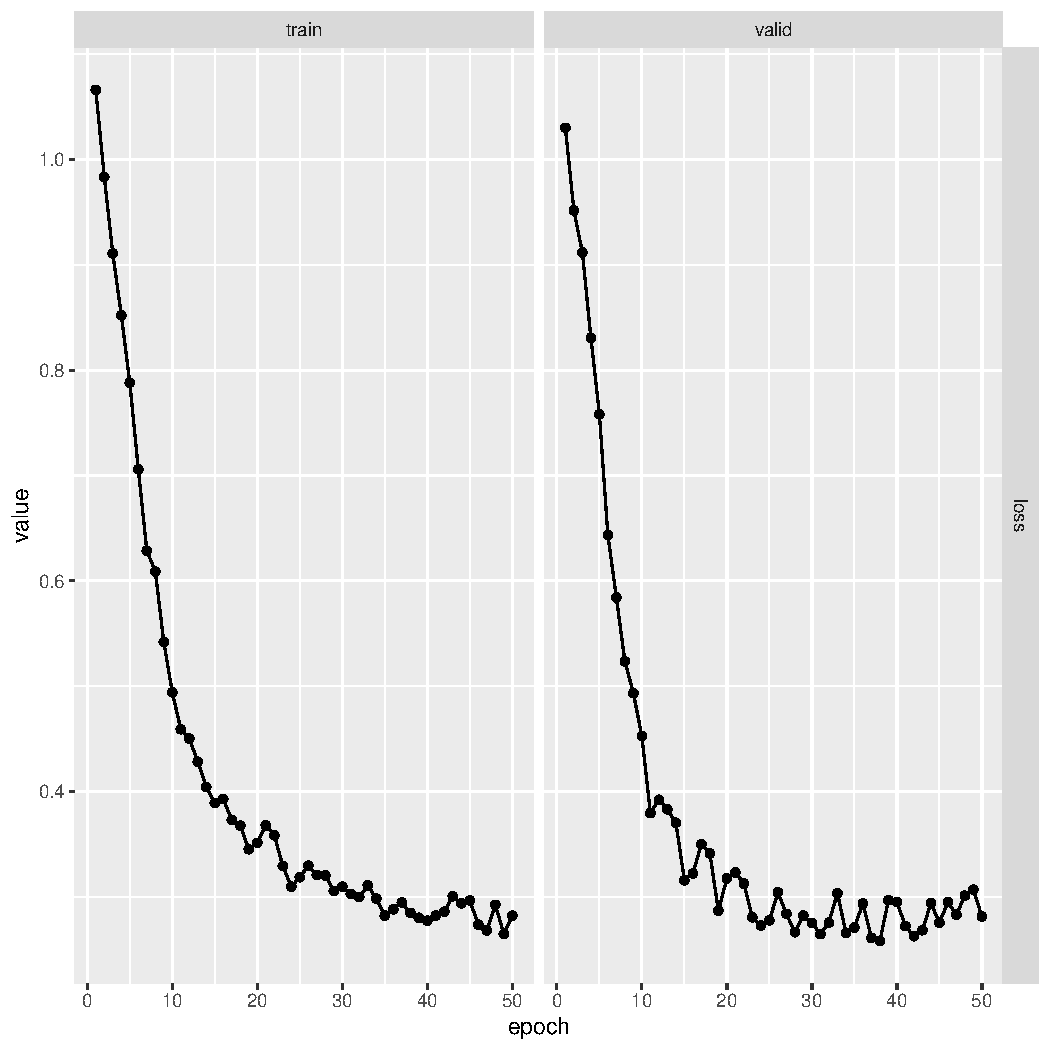
\includegraphics{hw5_files/figure-pdf/unnamed-chunk-37-1.pdf}

}

\end{figure}

\begin{Shaded}
\begin{Highlighting}[]
\CommentTok{\# 生成预测并绘制决策边界}
\NormalTok{test\_matrix }\OtherTok{\textless{}{-}}\NormalTok{ df\_test }\SpecialCharTok{\%\textgreater{}\%} \FunctionTok{select}\NormalTok{(x1, x2) }\SpecialCharTok{\%\textgreater{}\%} \FunctionTok{as.matrix}\NormalTok{()}
\NormalTok{fit\_3\_predictions }\OtherTok{\textless{}{-}} \FunctionTok{predict}\NormalTok{(fit\_3, test\_matrix) }\SpecialCharTok{\%\textgreater{}\%}
  \FunctionTok{torch\_argmax}\NormalTok{(}\AttributeTok{dim =} \DecValTok{2}\NormalTok{) }\SpecialCharTok{\%\textgreater{}\%}
  \FunctionTok{as.integer}\NormalTok{()}

\FunctionTok{plot\_decision\_boundary}\NormalTok{(fit\_3\_predictions)}
\end{Highlighting}
\end{Shaded}

\begin{figure}[H]

{\centering 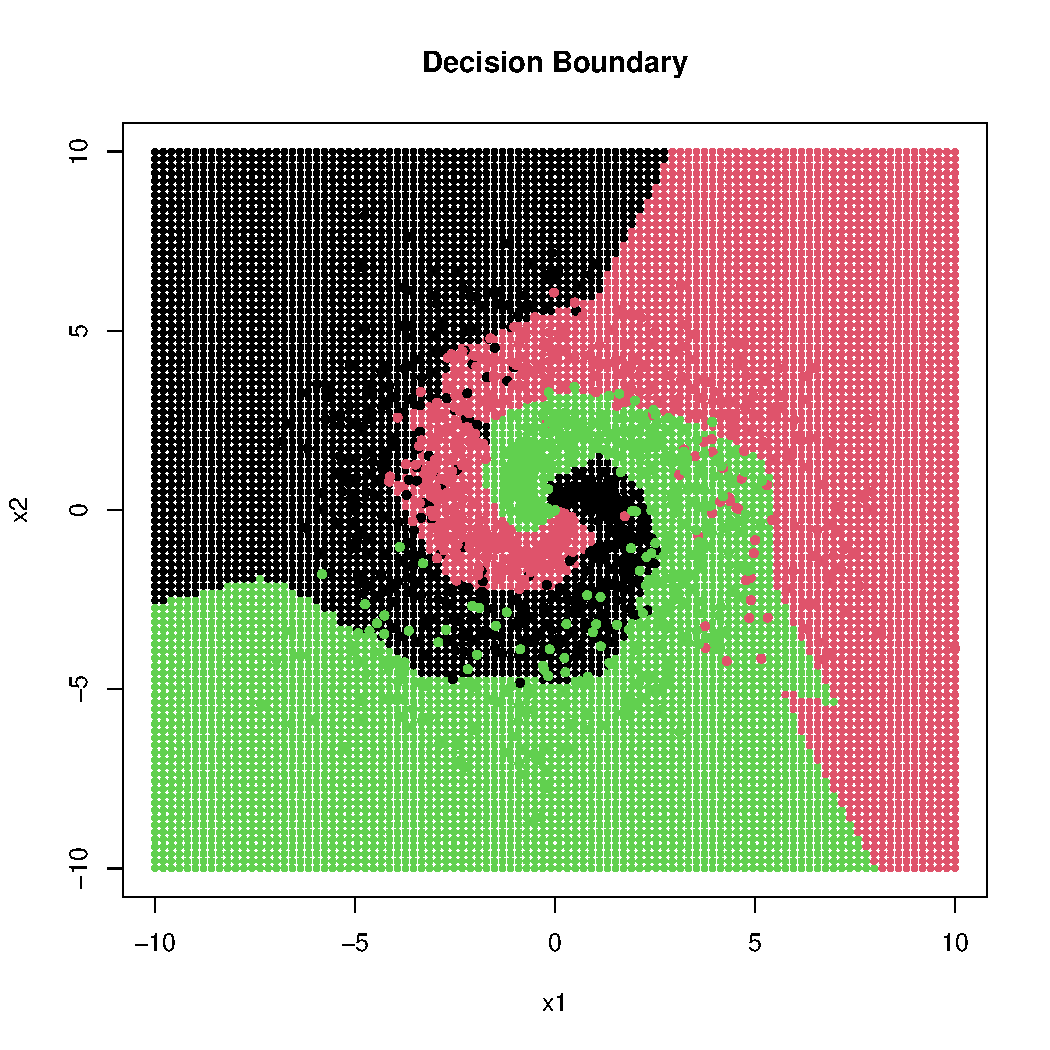
\includegraphics{hw5_files/figure-pdf/unnamed-chunk-37-2.pdf}

}

\end{figure}

\begin{center}\rule{0.5\linewidth}{0.5pt}\end{center}

3.7 (5 points)

What are the differences between the models? How do the decision
boundaries change as the number of hidden layers increases?

\begin{center}\rule{0.5\linewidth}{0.5pt}\end{center}

\pagebreak

---

\begin{tcolorbox}[enhanced jigsaw, bottomtitle=1mm, rightrule=.15mm, left=2mm, colback=white, opacityback=0, bottomrule=.15mm, titlerule=0mm, toprule=.15mm, colframe=quarto-callout-note-color-frame, arc=.35mm, colbacktitle=quarto-callout-note-color!10!white, breakable, leftrule=.75mm, coltitle=black, title=\textcolor{quarto-callout-note-color}{\faInfo}\hspace{0.5em}{Session Information}, opacitybacktitle=0.6, toptitle=1mm]

Print your \texttt{R} session information using the following command

\begin{Shaded}
\begin{Highlighting}[]
\CommentTok{\# sessionInfo()}
\end{Highlighting}
\end{Shaded}

\end{tcolorbox}



\end{document}
